\documentclass{article}
\usepackage[preprint]{neurips_2026}

\usepackage{amsmath}
\usepackage{amssymb}
\usepackage{booktabs}
\usepackage{graphicx}
\usepackage{subcaption}
\usepackage{microtype}
\usepackage{url}
\usepackage{float}
\usepackage{siunitx}
\usepackage{placeins}

\graphicspath{{outputs/figures/}{AlphaEarth/outputs/figures/}{../outputs/figures/}{../AlphaEarth/outputs/figures/}}

\title{Using AlphaEarth and Spatiotemporal Models to Detect Urban Cooling\\
from Chengdu's Park-City Policy}

\author{%
  Mengxiang (Louis) Liu \\
  EPS-210: AI for Earth and Planetary Science \\
  Harvard University \\
  April 2026 \\
  \small Code repository: \url{https://github.com/louis1mx/E-PSCI210}
}

\begin{document}
\maketitle

\begin{abstract}
Evaluating whether a specific urban greening policy produced measurable cooling
is difficult: land surface temperature (LST) is simultaneously affected by
weather variability, seasonal cycles, regional warming, and cloud-driven data
gaps that leave many months unusable in optical archives. Standard interrupted
time series approaches collapse these spatially heterogeneous effects into a
single city-wide average, discarding the spatial fingerprint that localized
greening would produce.

This paper proposes and implements a dual-layer AI framework to address these
limitations, applied to Chengdu, China, the first National Park-City
Demonstration Zone, designated in January 2022. First, a ConvLSTM model
trained only on pre-policy Landsat LST sequences serves as a learned
spatiotemporal reference: post-policy residuals identify pixels that cooled
beyond what pre-policy dynamics predict. Second, AlphaEarth Foundation
embeddings, annual 64-band multi-sensor representations at 10~m resolution, provide a surface-change verification layer, testing whether locations with
thermal anomalies also experienced detectable land-surface transformation
between 2021 and 2025.

The ITS model finds no significant city-wide cooling trend
($\beta_3 = +0.047$~$^\circ$C/month, $p = 0.574$). The ConvLSTM outperforms
seasonal climatology (RMSE 4.10 vs.\ 4.34~$^\circ$C) and reveals localized
cooling residuals in western, southwestern, and southeastern Chengdu. AlphaEarth embedding
change is weakly correlated with cooling residuals ($r = 0.071$) and
$\Delta$NDVI ($r = 0.112$), and negatively correlated with $\Delta$LST
($r = -0.124$). Only 6.3\% of grid cells fall into the joint high-change plus
high-cooling quadrant (Jaccard = 0.143), with high-change cells roughly evenly
split between cooling and warming. Rather than overstating policy success, the
framework reveals where Chengdu changed, where it cooled, and crucially, where
those signals do not agree. It serves as a more honest foundation for causal attribution
than LST alone.
\end{abstract}

\section{Introduction}
\label{sec:intro}

Urban heat islands are an important climate and public health problem. Dense
cities replace vegetation with buildings, roads, and other impervious surfaces,
which increases land surface temperature (LST), heat exposure, and cooling
demand \citep{Oke1982, Zhao2014}. Many cities are now using parks, greenways,
tree planting, and blue-green infrastructure as nature-based solutions. These
policies are attractive because they can provide cooling while also improving
air quality, stormwater management, and quality of life. However, the empirical
question is difficult: after a city invests in greening, can we actually detect
a cooling signal from satellite data?

This paper studies Chengdu, a large city in the Sichuan Basin. Chengdu was
designated China's first National Park-City Demonstration Zone in January 2022.
Before and around this designation, the city invested in community parks,
greenways, and ecological corridors. This makes Chengdu a useful case for
testing whether urban greening policy can produce measurable cooling. The
policy date provides a clear before/after structure, but isolating a causal
cooling signal is complicated by strong seasonality, persistent cloud
contamination, and regional warming during the post-policy period. A simple
comparison of average temperature before and after 2022 is therefore not enough.

This paper combines three methods. Interrupted time series (ITS) regression
tests whether average urban LST changed after the January 2022 policy start
while controlling for weather and month fixed effects. A ConvLSTM model trained
only on pre-policy Landsat images generates a spatiotemporal reference against
which post-policy observations are compared. The ITS model does not find
statistically significant city-wide cooling. The ConvLSTM residual maps,
however, suggest localized cooling in western, southwestern, and southeastern Chengdu,
indicating that the policy signal may be spatially heterogeneous rather than
a uniform city-level shift.

The third contribution is a surface-change verification layer using AlphaEarth
Foundations embeddings. AlphaEarth is a geospatial foundation model that
produces annual satellite
embeddings from multi-sensor Earth observation data \citep{Brown2025,
Google2025Catalog}. Each 10 m pixel is represented by a 64-dimensional
embedding summarizing spectral, spatial, and temporal information. These
embeddings are designed for downstream tasks such as classification, regression,
similarity search, and change detection. For this project, AlphaEarth is
important because it can help answer a question that LST alone cannot answer:
did the places that cooled also experience meaningful surface-form change?

The paper therefore asks four questions:
\begin{enumerate}
  \item Did Chengdu's city-wide LST trajectory change after the January 2022
  Park-City policy designation?
  \item Are post-policy temperatures cooler than a ConvLSTM counterfactual
  learned from pre-policy spatial-temporal patterns?
  \item Can AlphaEarth annual embeddings provide an additional change detection
  signal that helps identify where urban surface form changed?
  \item Do AlphaEarth change hotspots align more closely with cooling,
  vegetation gain, or warming?
\end{enumerate}

The AlphaEarth analysis focuses on a single embedding-change map for Chengdu,
aligned with the ConvLSTM residual map and interpreted using annual
$\Delta$LST and $\Delta$NDVI layers.

\section{Data}
\label{sec:data}

\subsection{Study Area}

The study area is Chengdu, China. The urban zone is defined as a 25 km buffer
around Tianfu Square, the central point of the city. A 25--50 km annular ring
is used as a rural reference zone for urban heat island benchmarking. This
simple geometry is not perfect, because the rural ring can still include
peri-urban development, but it gives a consistent way to compare the urban core
with a less dense surrounding area.

\subsection{Landsat Land Surface Temperature}

The main temperature dataset is Landsat 8/9 Collection 2 Level-2 surface
temperature. I use the \texttt{ST\_B10} band and convert it to degrees Celsius
using the product scale and offset. Cloud and shadow pixels are masked with the
\texttt{QA\_PIXEL} band. Monthly median composites are created in Google Earth
Engine for January 2016 through December 2025.

The final Landsat archive contains 109 monthly LST composites. This is less
than the full 120 months because several months have missing or unusable data.
Coverage is a major limitation. Sichuan Basin cloud cover and the Landsat
16-day revisit cycle make the monthly image stack uneven. Some months have good
coverage, while others require interpolation or have large areas with missing
pixels. This limitation matters directly for the AlphaEarth comparison because
annual $\Delta$LST inherits the same spatial gaps.

\subsection{Vegetation and Weather Controls}

I use MODIS NDVI as a vegetation indicator and ERA5 reanalysis as weather
controls. ERA5 variables include 2 m air temperature, precipitation, and
shortwave radiation. These controls are included because urban LST can change
because of weather alone. Without weather controls, post-2022 regional warming
could be incorrectly interpreted as a failure of the greening policy.

\subsection{AlphaEarth Satellite Embeddings}

The AlphaEarth Foundations Satellite Embedding dataset provides annual 10 m,
64-band embedding images produced from AlphaEarth Foundations
\citep{Google2025Catalog}. The embeddings are generated from
multiple Earth observation streams, including optical and radar sensors, and
are meant to be used as analysis-ready features. Google Earth Engine tutorials
explicitly list change detection as one of the downstream uses of the embeddings
\citep{Google2025Tutorial}.

For this Chengdu pilot, I export annual AlphaEarth embeddings for 2017--2025
and aggregate them to the same $64 \times 64$ grid used by the ConvLSTM model.
I also export annual NDVI rasters to the same grid so that AlphaEarth change can
be compared not only with ConvLSTM residuals but also with an interpretable
vegetation layer.

\begin{table}[H]
\caption{Datasets used in the Chengdu analysis.}
\label{tab:data_summary}
\centering
\small
\begin{tabular}{lccc}
\toprule
\textbf{Dataset} & \textbf{Resolution} & \textbf{Period} & \textbf{Use} \\
\midrule
Landsat 8/9 LST & 30 m & 2016--2025 & Temperature outcome \\
MODIS NDVI & 250 m & 2016--2025 & Vegetation trend and annual $\Delta$NDVI \\
ERA5 reanalysis & 0.25 degree & 2016--2025 & Weather controls \\
AlphaEarth embeddings & 10 m & annual, 2017--2025 & Change detection and greening classification \\
ESA WorldCover & 10 m & 2021 & Land-cover labels for embedding classifier \\
\bottomrule
\end{tabular}
\end{table}

\subsection{ESA WorldCover Land-Cover Labels}

ESA WorldCover v200 provides a global 10 m land-cover classification map for
2021 \citep{Zanaga2022}. The map assigns each pixel to one of ten classes
including tree cover, shrubland, grassland, cropland, built-up, bare land, and
water bodies. For this analysis, classes are collapsed into three groups:
\textit{vegetation} (tree cover, shrubland, grassland, wetlands), \textit{built}
(built-up), and \textit{other} (cropland, bare, water). The 2021 WorldCover map
is exported from Google Earth Engine onto the same $64 \times 64$ analysis grid
and used as ground-truth labels to train the embedding classifier described in
Section~\ref{sec:worldcover_method}.

\section{Methods}
\label{sec:methods}

\subsection{Interrupted Time Series Regression}

The first method is interrupted time series regression \citep{Bernal2017}. This
model estimates whether there is a city-wide change in mean urban LST after
January 2022. The
regression is:
\begin{equation}
\mathrm{LST}_t = \alpha + \beta_1 t + \beta_3 D_t(t-T_0)
+ \boldsymbol{\gamma}^{\top}\mathbf{X}_t + \boldsymbol{\delta}_m M_m
+ \varepsilon_t,
\end{equation}
where $D_t$ is a post-policy indicator, $T_0$ is the policy start time,
$\mathbf{X}_t$ includes ERA5 weather controls, and $M_m$ are month fixed
effects. The coefficient $\beta_3$ measures a post-policy trend change.
An immediate level-shift term is excluded because a greening policy cannot
plausibly produce an instantaneous city-wide temperature jump on the first
day of designation. I use HC3 robust standard errors because the sample is
not large and residual variance may not be constant \citep{MacKinnon1985}.

This model is useful because it is interpretable. It directly tests whether the
average city became cooler after the policy. However, it has an important
weakness: it collapses the city into one monthly number. If only some districts
or corridors cool, the effect can disappear in the average.

\subsection{ConvLSTM Counterfactual Model}

The second method is a ConvLSTM spatiotemporal model \citep{Shi2015}. The model
is trained on pre-policy LST image sequences to learn the pre-policy
spatiotemporal distribution of urban LST. This learned distribution is then
used as a reference against which post-policy observations are compared.
This differs from strict forecasting: the model learns the spatial-temporal
structure of pre-policy LST, not a causal model of future conditions. The
comparison is interpreted as a counterfactual reference: what the city would
have looked like after 2022 if pre-policy dynamics had continued.

The residual is:
\begin{equation}
R_{i,t} = \widehat{Y}_{i,t}^{counterfactual} - Y_{i,t}^{observed}.
\label{eq:residual}
\end{equation}
If $R_{i,t}$ is positive, the observed LST is cooler than the model expected at
pixel $i$ and month $t$. This does not prove the policy caused the cooling, but
it identifies where cooling is stronger than expected from historical patterns.

The ConvLSTM takes as input 12 consecutive monthly LST images
(each resampled to $64 \times 64$ pixels) and predicts the next month's LST
image (a one-step-ahead forecast in the temporal sequence). The model has two
ConvLSTM layers and a convolutional output head. It is trained only on
pre-policy monthly images (January 2016 -- December 2021, 60 months), using the
first 48 months for training and the remaining 12 as a validation set. The
46 post-policy months (January 2022 -- October 2025) are held out entirely for
evaluation. For the AlphaEarth alignment analysis, I use the mean residual
across all post-policy months.

\subsection{AlphaEarth Change Detection}

The AlphaEarth analysis is implemented in three steps.

First, I compute annual embedding change by comparing a pre-policy year (2021)
with a post-policy year (2025). The baseline metric is cosine distance:
\begin{equation}
\Delta E_i = 1 - \cos(E_{i,2021}, E_{i,2025}),
\label{eq:cosine}
\end{equation}
where $E_i$ is the 64-dimensional AlphaEarth vector at location $i$. Larger
values mean larger semantic change in the satellite embedding space.

Second, I compare $\Delta E_i$ with the ConvLSTM cooling residual, annual mean
$\Delta$LST, and annual mean $\Delta$NDVI. The annual mean LST difference is
computed as:
\begin{equation}
\Delta \mathrm{LST}_i = \overline{\mathrm{LST}}_{i,2025} - \overline{\mathrm{LST}}_{i,2021},
\label{eq:dlst}
\end{equation}
and the annual NDVI difference is:
\begin{equation}
\Delta \mathrm{NDVI}_i = \mathrm{NDVI}_{i,2025} - \mathrm{NDVI}_{i,2021}.
\label{eq:dndvi}
\end{equation}
I then compute cell-wise Pearson correlations between embedding change and each
of these layers.

Third, I create a quadrant map by crossing the WorldCover-supervised greening
probability change ($\Delta$greening\_prob, described in
Section~\ref{sec:worldcover_method}) with the ConvLSTM cooling residual, using
the 75th percentile of each distribution as thresholds. This creates four
interpretable categories:
\begin{itemize}
  \item greening and cooling (the strongest policy-consistent signal);
  \item greening and warming (surface transformation without thermal benefit);
  \item paving and cooling (cooling despite surface change toward built form);
  \item paving and warming or background (development-consistent pattern).
\end{itemize}

\subsection{WorldCover-Supervised Embedding Interpretation}
\label{sec:worldcover_method}

To translate AlphaEarth embedding change into interpretable land-cover
transitions, I train a Random Forest classifier on the 2021 AlphaEarth
embeddings using ESA WorldCover 2021 as ground-truth labels. Each valid
$64 \times 64$ grid cell provides a 64-dimensional feature vector (the
AlphaEarth embedding) and a three-class label (vegetation, built, other)
derived from the dominant WorldCover class within that cell.

The classifier is evaluated using 5-fold stratified cross-validation
(accuracy = 0.758), indicating that AlphaEarth embeddings carry sufficient
land-cover information at the analysis grid resolution. The trained classifier
is then applied to the 2025 AlphaEarth embeddings to predict land-cover
probabilities for the post-policy year. The greening probability change is
defined as:
\begin{equation}
\Delta\text{greening\_prob}_i =
  P(\text{vegetation} \mid E_{i,2025}) - P(\text{vegetation} \mid E_{i,2021}),
\label{eq:dgreening}
\end{equation}
where positive values indicate that a cell's embedding shifted toward
vegetation-like patterns (greening) and negative values indicate a shift toward
built or bare land (paving).

\section{Results}
\label{sec:results}

\subsection{Descriptive Patterns}

The Landsat data show strong seasonality in both urban and rural LST. Urban
mean LST increased from 25.50$^\circ$C before 2022 to 26.62$^\circ$C after
2022. Rural LST also increased, from 24.53$^\circ$C to 25.50$^\circ$C. This
means that raw urban warming cannot be interpreted as policy failure, because
the whole region also warmed. Urban NDVI increased slightly from 0.475 to
0.483, which is consistent with greening but not strong enough by itself to
prove a policy effect.

\begin{figure}[H]
  \centering
  \begin{subfigure}[b]{0.48\linewidth}
    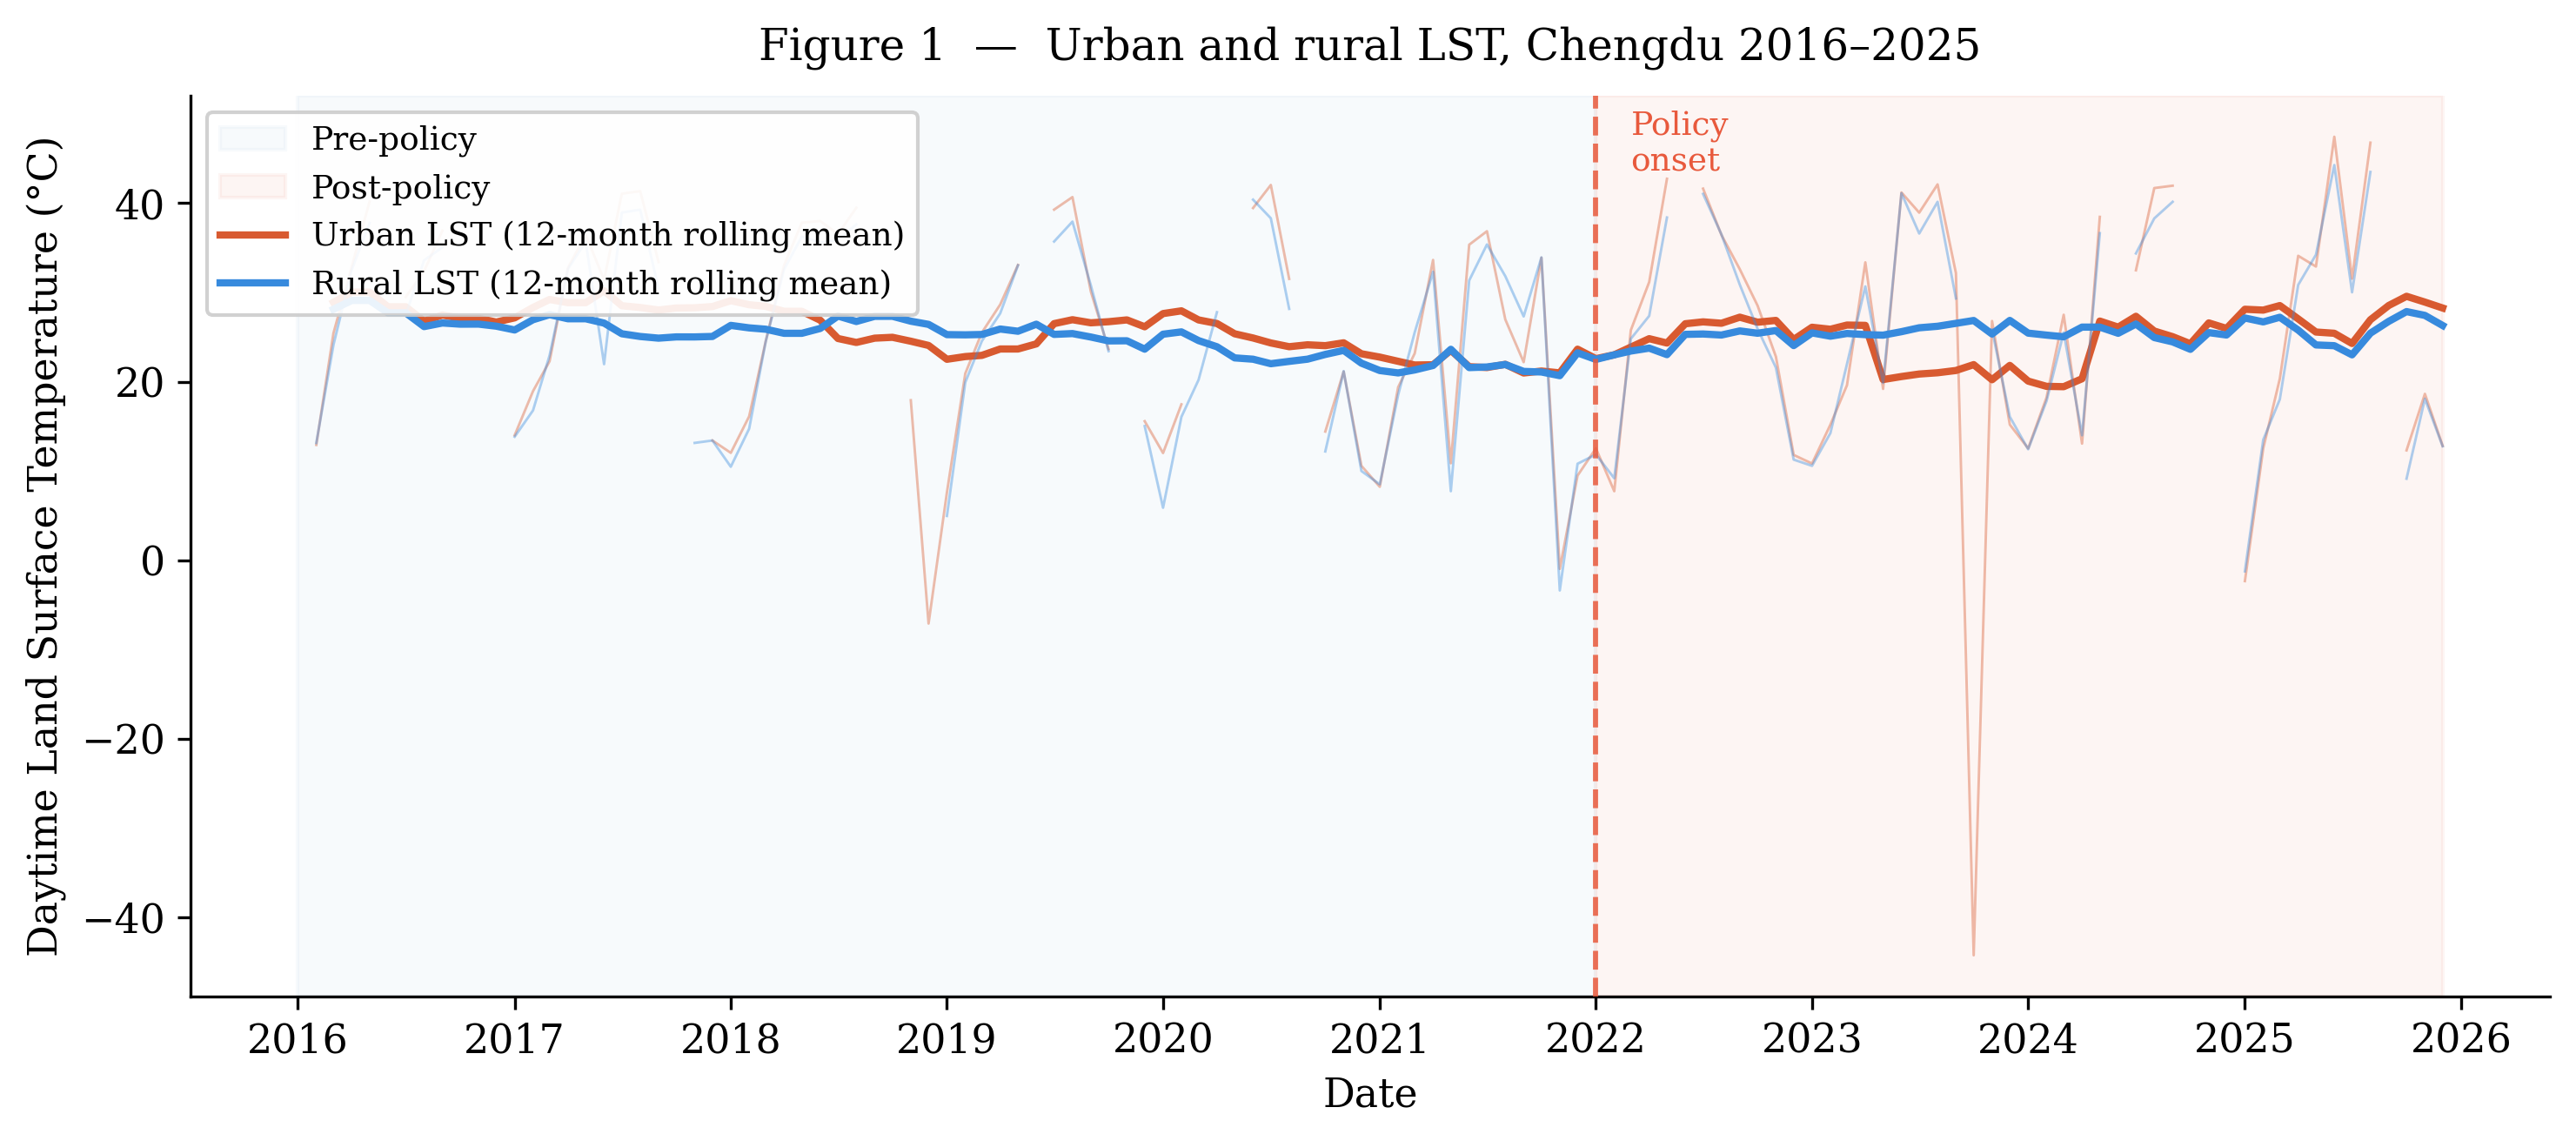
\includegraphics[width=\linewidth]{fig1_lst_trend.png}
    \caption{Urban and rural LST.}
  \end{subfigure}\hfill
  \begin{subfigure}[b]{0.48\linewidth}
    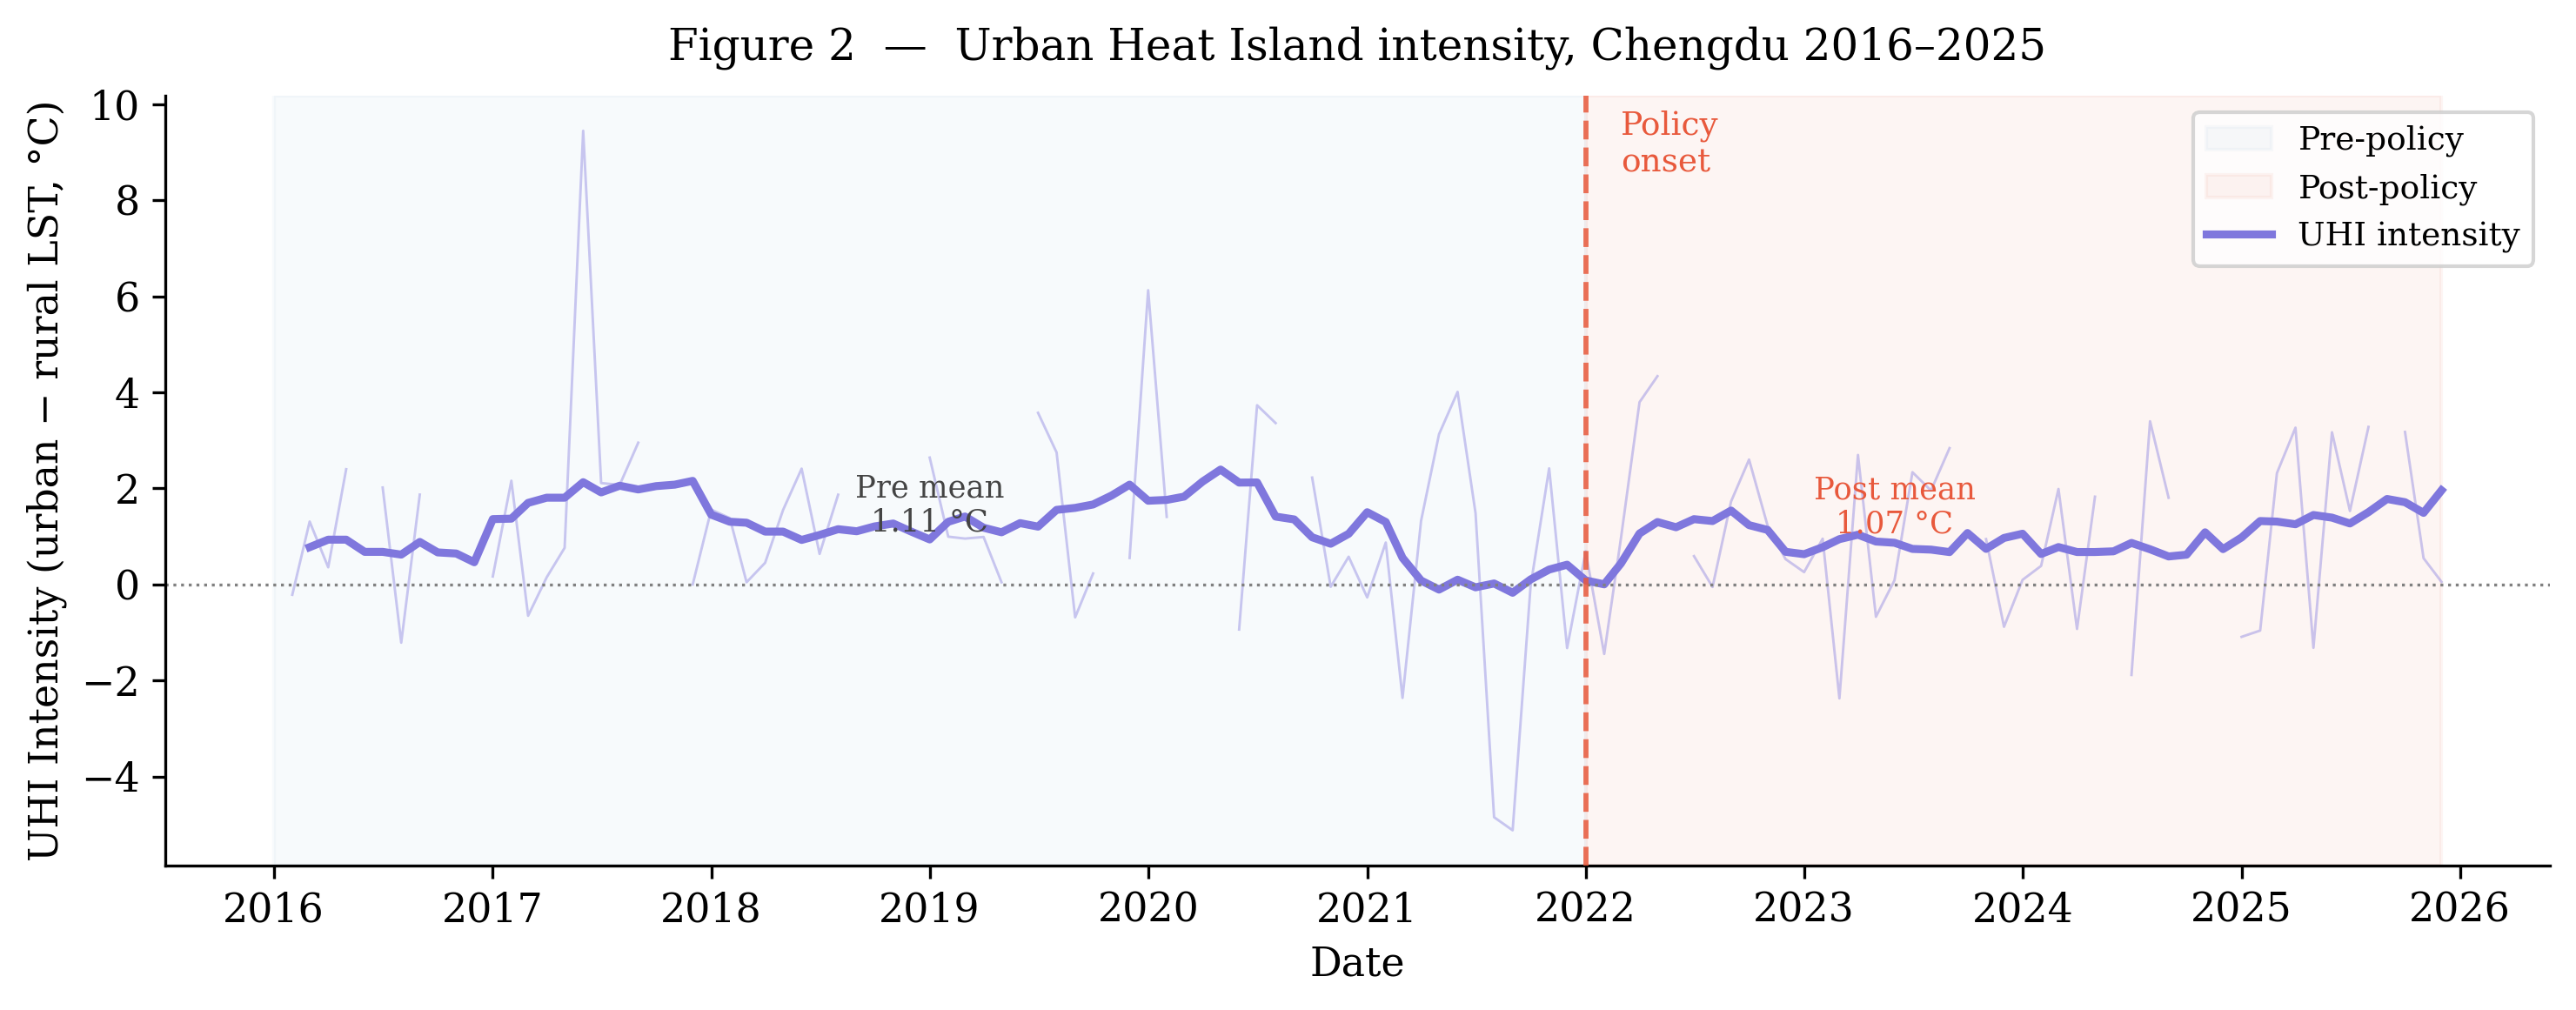
\includegraphics[width=\linewidth]{fig2_uhi_trend.png}
    \caption{Urban-rural thermal contrast.}
  \end{subfigure}
  \caption{Monthly LST and UHI trends from 2016 to 2025. The dashed line marks
  the January 2022 policy date.}
  \label{fig:trends}
\end{figure}

\begin{figure}[H]
  \centering
  \begin{subfigure}[b]{0.48\linewidth}
    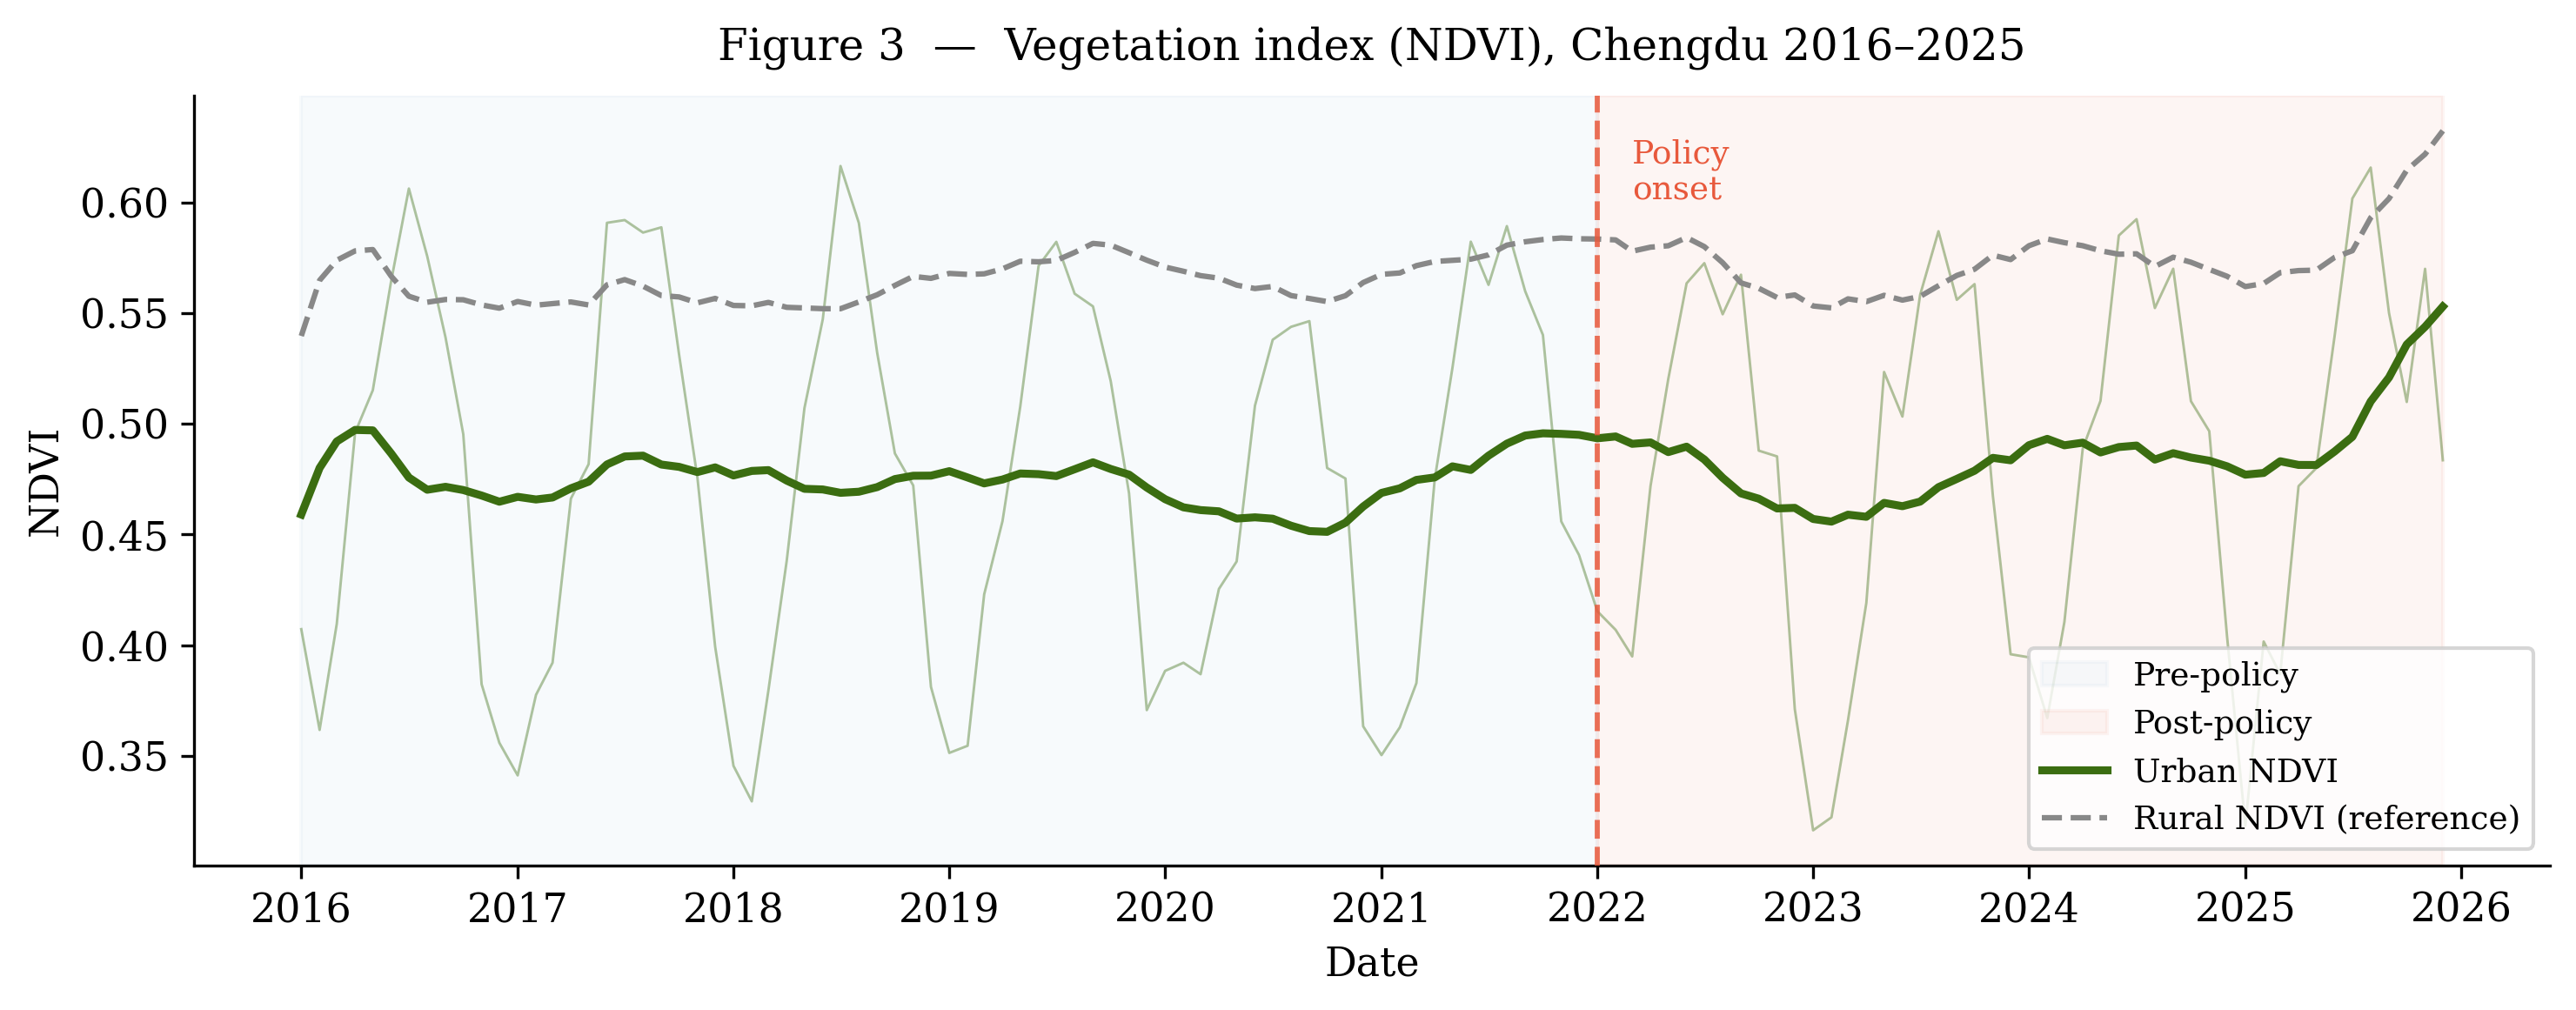
\includegraphics[width=\linewidth]{fig3_ndvi_trend.png}
    \caption{NDVI trend.}
  \end{subfigure}\hfill
  \begin{subfigure}[b]{0.48\linewidth}
    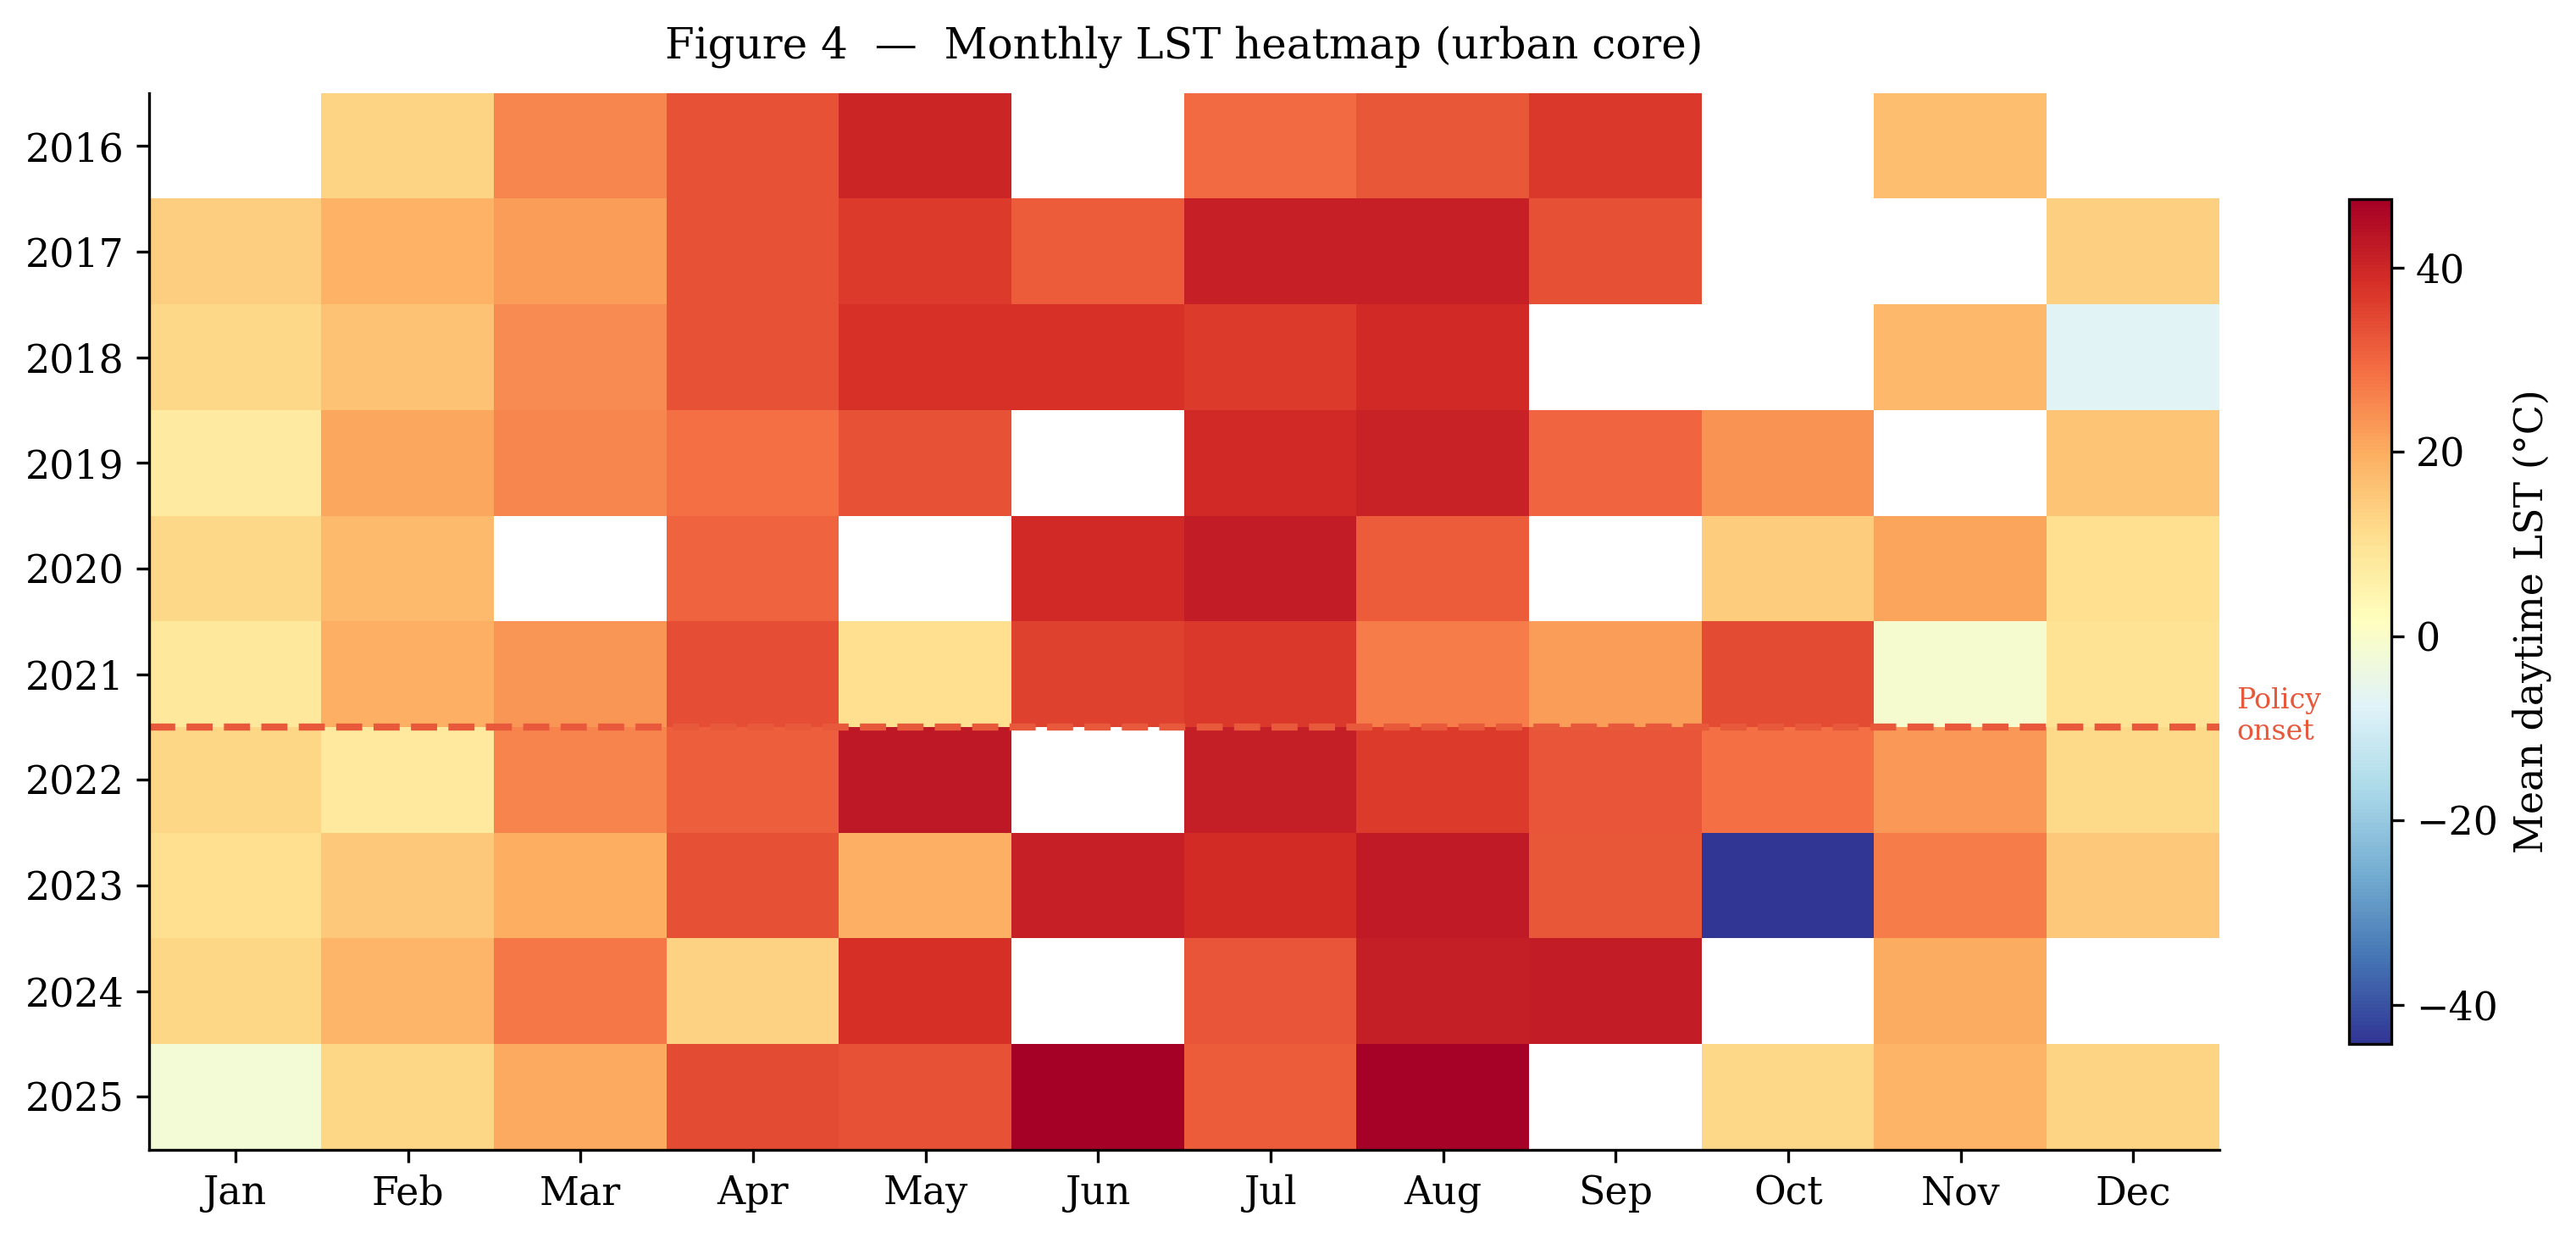
\includegraphics[width=\linewidth]{fig4_seasonal_heatmap.png}
    \caption{Seasonal LST heatmap.}
  \end{subfigure}
  \caption{Vegetation and seasonal diagnostics.}
  \label{fig:ndvi}
\end{figure}

\subsection{Interrupted Time Series Results}

The ITS model explains a large amount of monthly LST variation
($R^2=0.767$), mostly because seasonality and weather are strong predictors.
The post-policy slope change is near zero and not statistically significant
($\beta_3 = +0.047$~$^\circ$C/month, $p=0.574$). At the 5 percent
significance level, the ITS model does not support a detectable city-average
cooling trend after January 2022.

\begin{table}[H]
\caption{Key ITS coefficients from the current Chengdu model (no immediate
level-shift term).}
\label{tab:its}
\centering
\small
\begin{tabular}{lcccc}
\toprule
\textbf{Term} & \textbf{Coef.} & \textbf{SE} & \textbf{$z$} & \textbf{$p$} \\
\midrule
Time trend & $-0.0312$ & 0.033 & $-0.933$ & 0.351 \\
Post-policy slope change & $+0.0469$ & 0.084 & $+0.562$ & 0.574 \\
ERA5 2m temperature & $+1.2976$ & 0.597 & $+2.173$ & 0.030 \\
Precipitation & $-0.0844$ & 0.288 & $-0.293$ & 0.770 \\
Shortwave radiation & $+0.0733$ & 1.203 & $+0.061$ & 0.951 \\
\bottomrule
\end{tabular}
\end{table}

This is not necessarily surprising. Greening effects may be localized and
gradual, and a slope-change model is a conservative test: it asks whether the
city's LST trajectory shifted over several years, not whether there was an
instantaneous break. This result motivates the spatial models.

\begin{figure}[H]
  \centering
  \begin{subfigure}[b]{0.48\linewidth}
    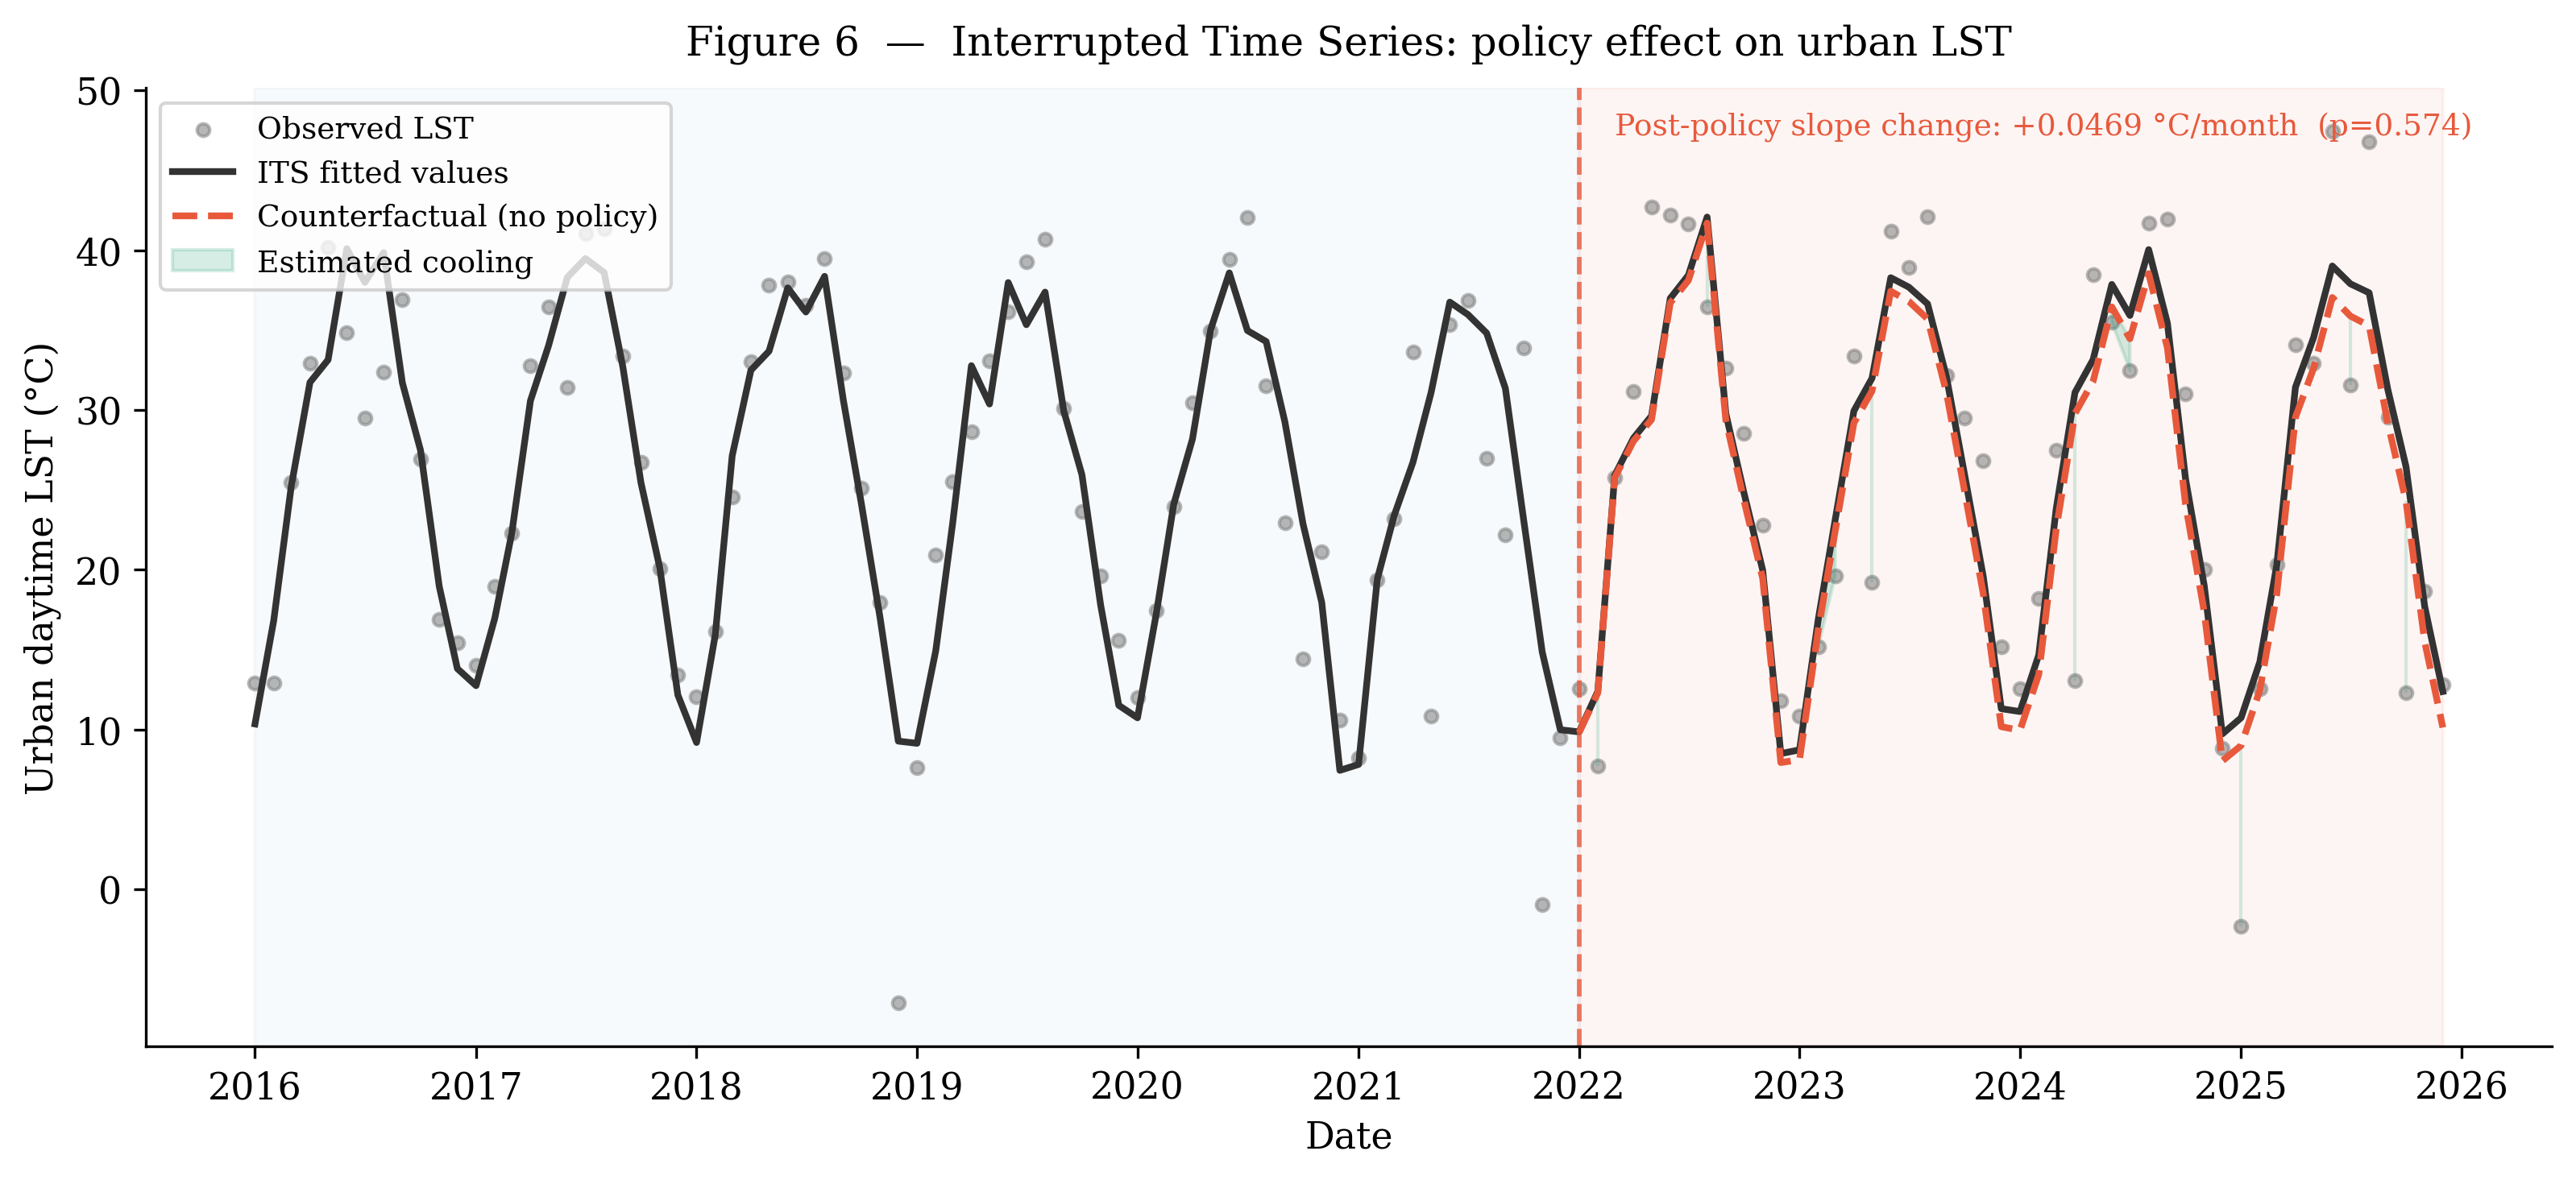
\includegraphics[width=\linewidth]{fig6_its_regression.png}
    \caption{Observed, fitted, and counterfactual LST.}
  \end{subfigure}\hfill
  \begin{subfigure}[b]{0.48\linewidth}
    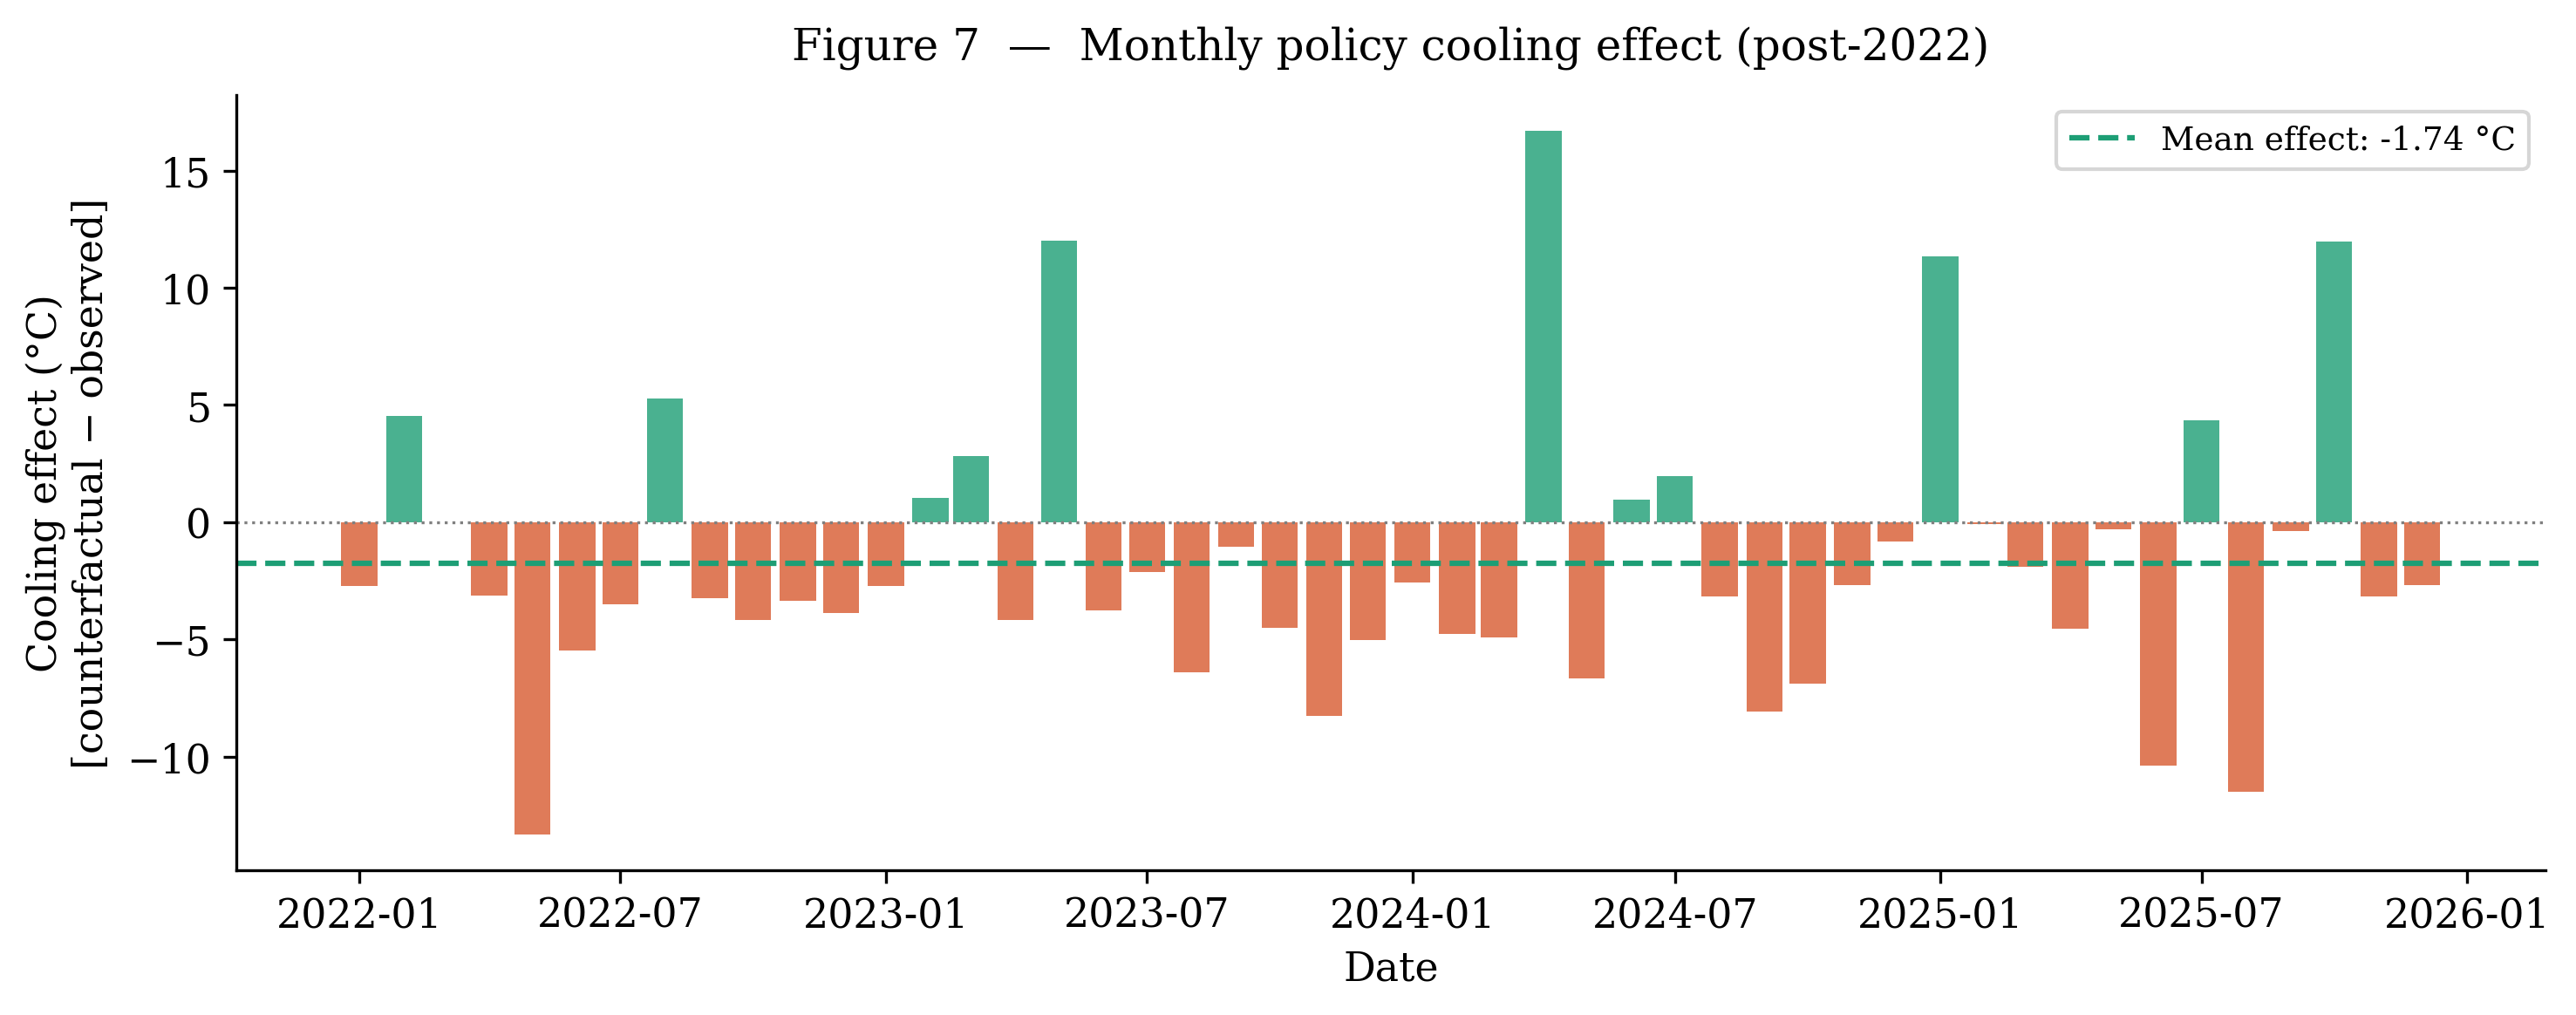
\includegraphics[width=\linewidth]{fig7_counterfactual.png}
    \caption{Counterfactual gap.}
  \end{subfigure}
  \caption{ITS counterfactual diagnostics.}
  \label{fig:its}
\end{figure}

\subsection{ConvLSTM Results}

The ConvLSTM achieves RMSE = 4.10$^\circ$C and MAE = 1.94$^\circ$C on
post-policy months. Table~\ref{tab:baseline} compares this against two naive
baselines evaluated on the same held-out months.

\begin{table}[H]
\caption{ConvLSTM vs.\ naive baselines on post-policy months (2022--2025).}
\label{tab:baseline}
\centering
\small
\begin{tabular}{lcc}
\toprule
\textbf{Model} & \textbf{RMSE ($^\circ$C)} & \textbf{MAE ($^\circ$C)} \\
\midrule
Persistence (2021 monthly mean) & 6.44 & 3.43 \\
Seasonal climatology & 4.34 & 2.20 \\
ConvLSTM & \textbf{4.10} & \textbf{1.94} \\
\bottomrule
\end{tabular}
\end{table}

The ConvLSTM outperforms both baselines, but its margin over seasonal
climatology is modest (0.24$^\circ$C RMSE). This is expected: aggregate
accuracy is not the model's primary contribution. Its value lies in
capturing spatial heterogeneity: which pixels cooled more than the pre-policy
pattern predicts, a signal that a spatially uniform climatology cannot produce. The spatial residual maps show that parts of western and
southwestern Chengdu are cooler than the pre-policy reference, consistent
with spatially concentrated greening effects.

\begin{figure}[H]
  \centering
  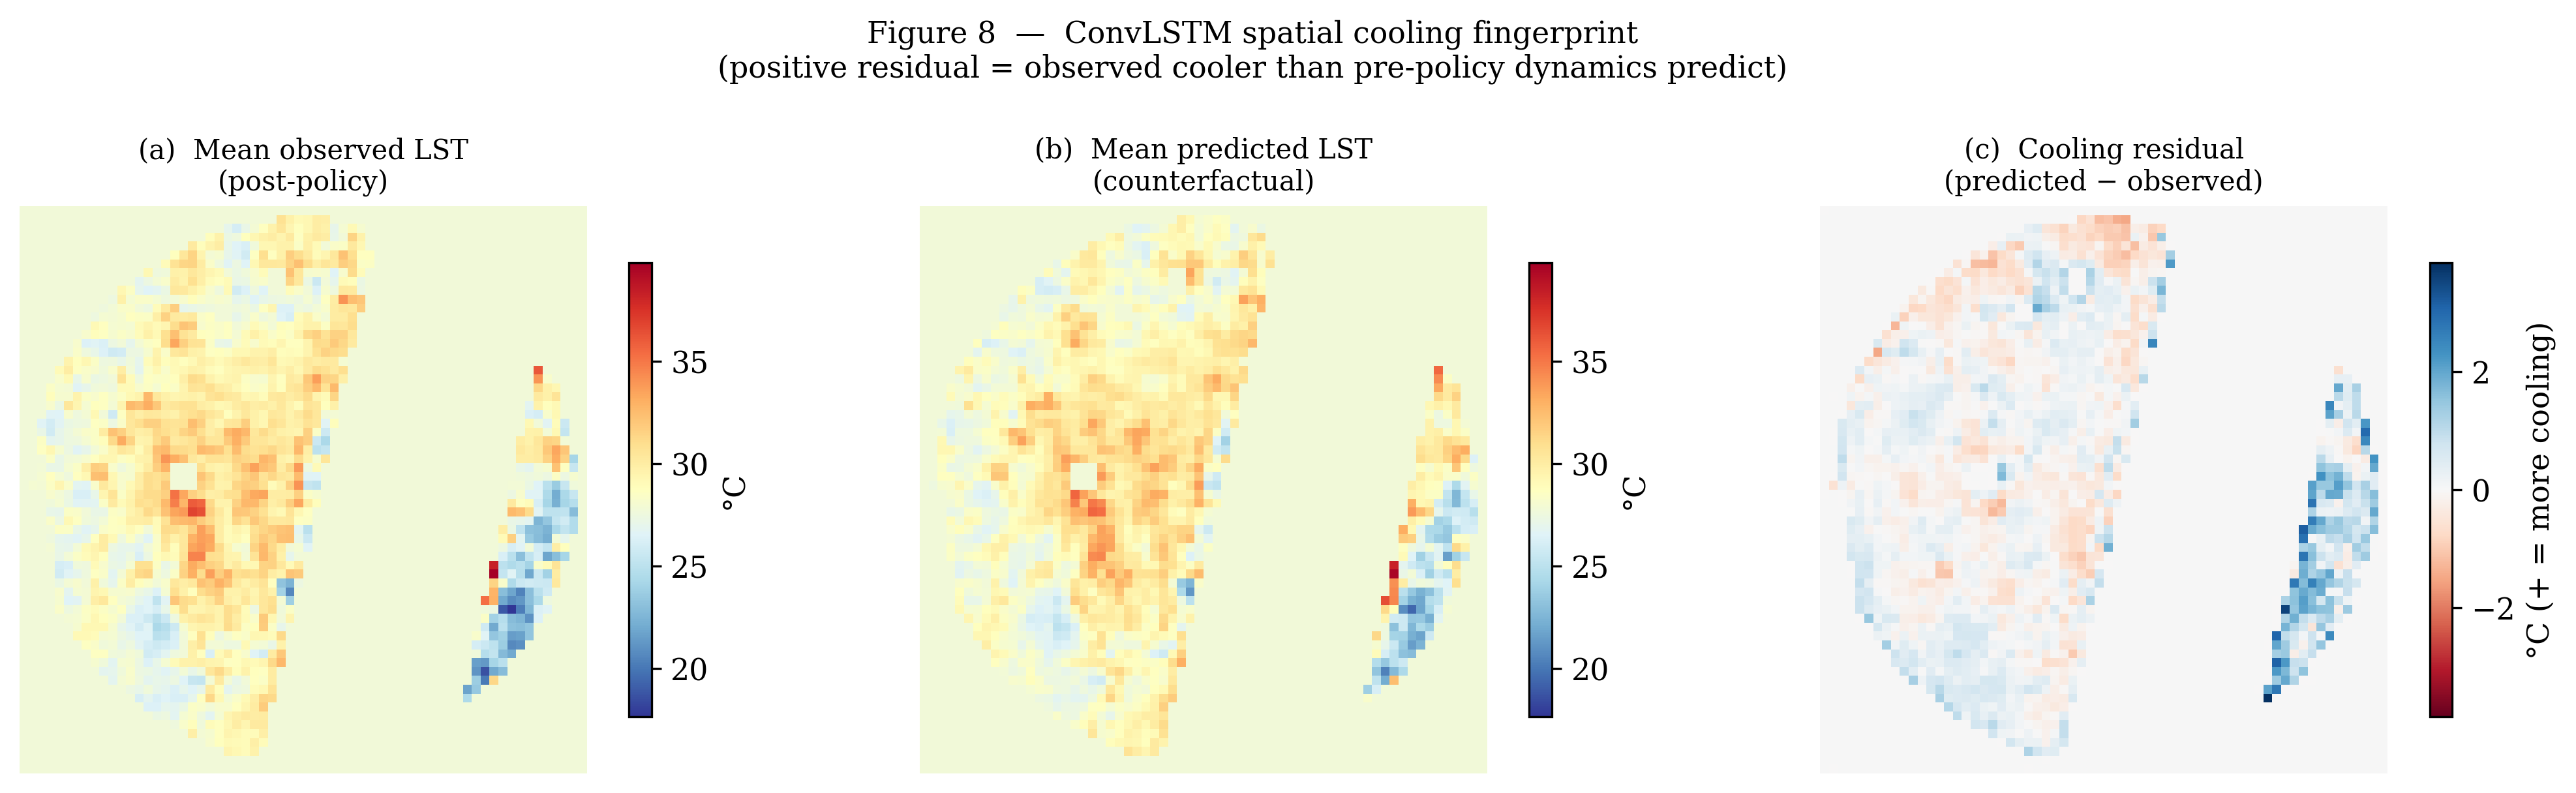
\includegraphics[width=0.68\linewidth]{fig8_convlstm_residuals.png}
  \caption{ConvLSTM spatial cooling residual map averaged over 2022--2025.
  Positive residuals indicate observed LST cooler than the pre-policy reference.}
  \label{fig:convlstm_map}
\end{figure}
\vspace{-4mm}
\begin{figure}[H]
  \centering
  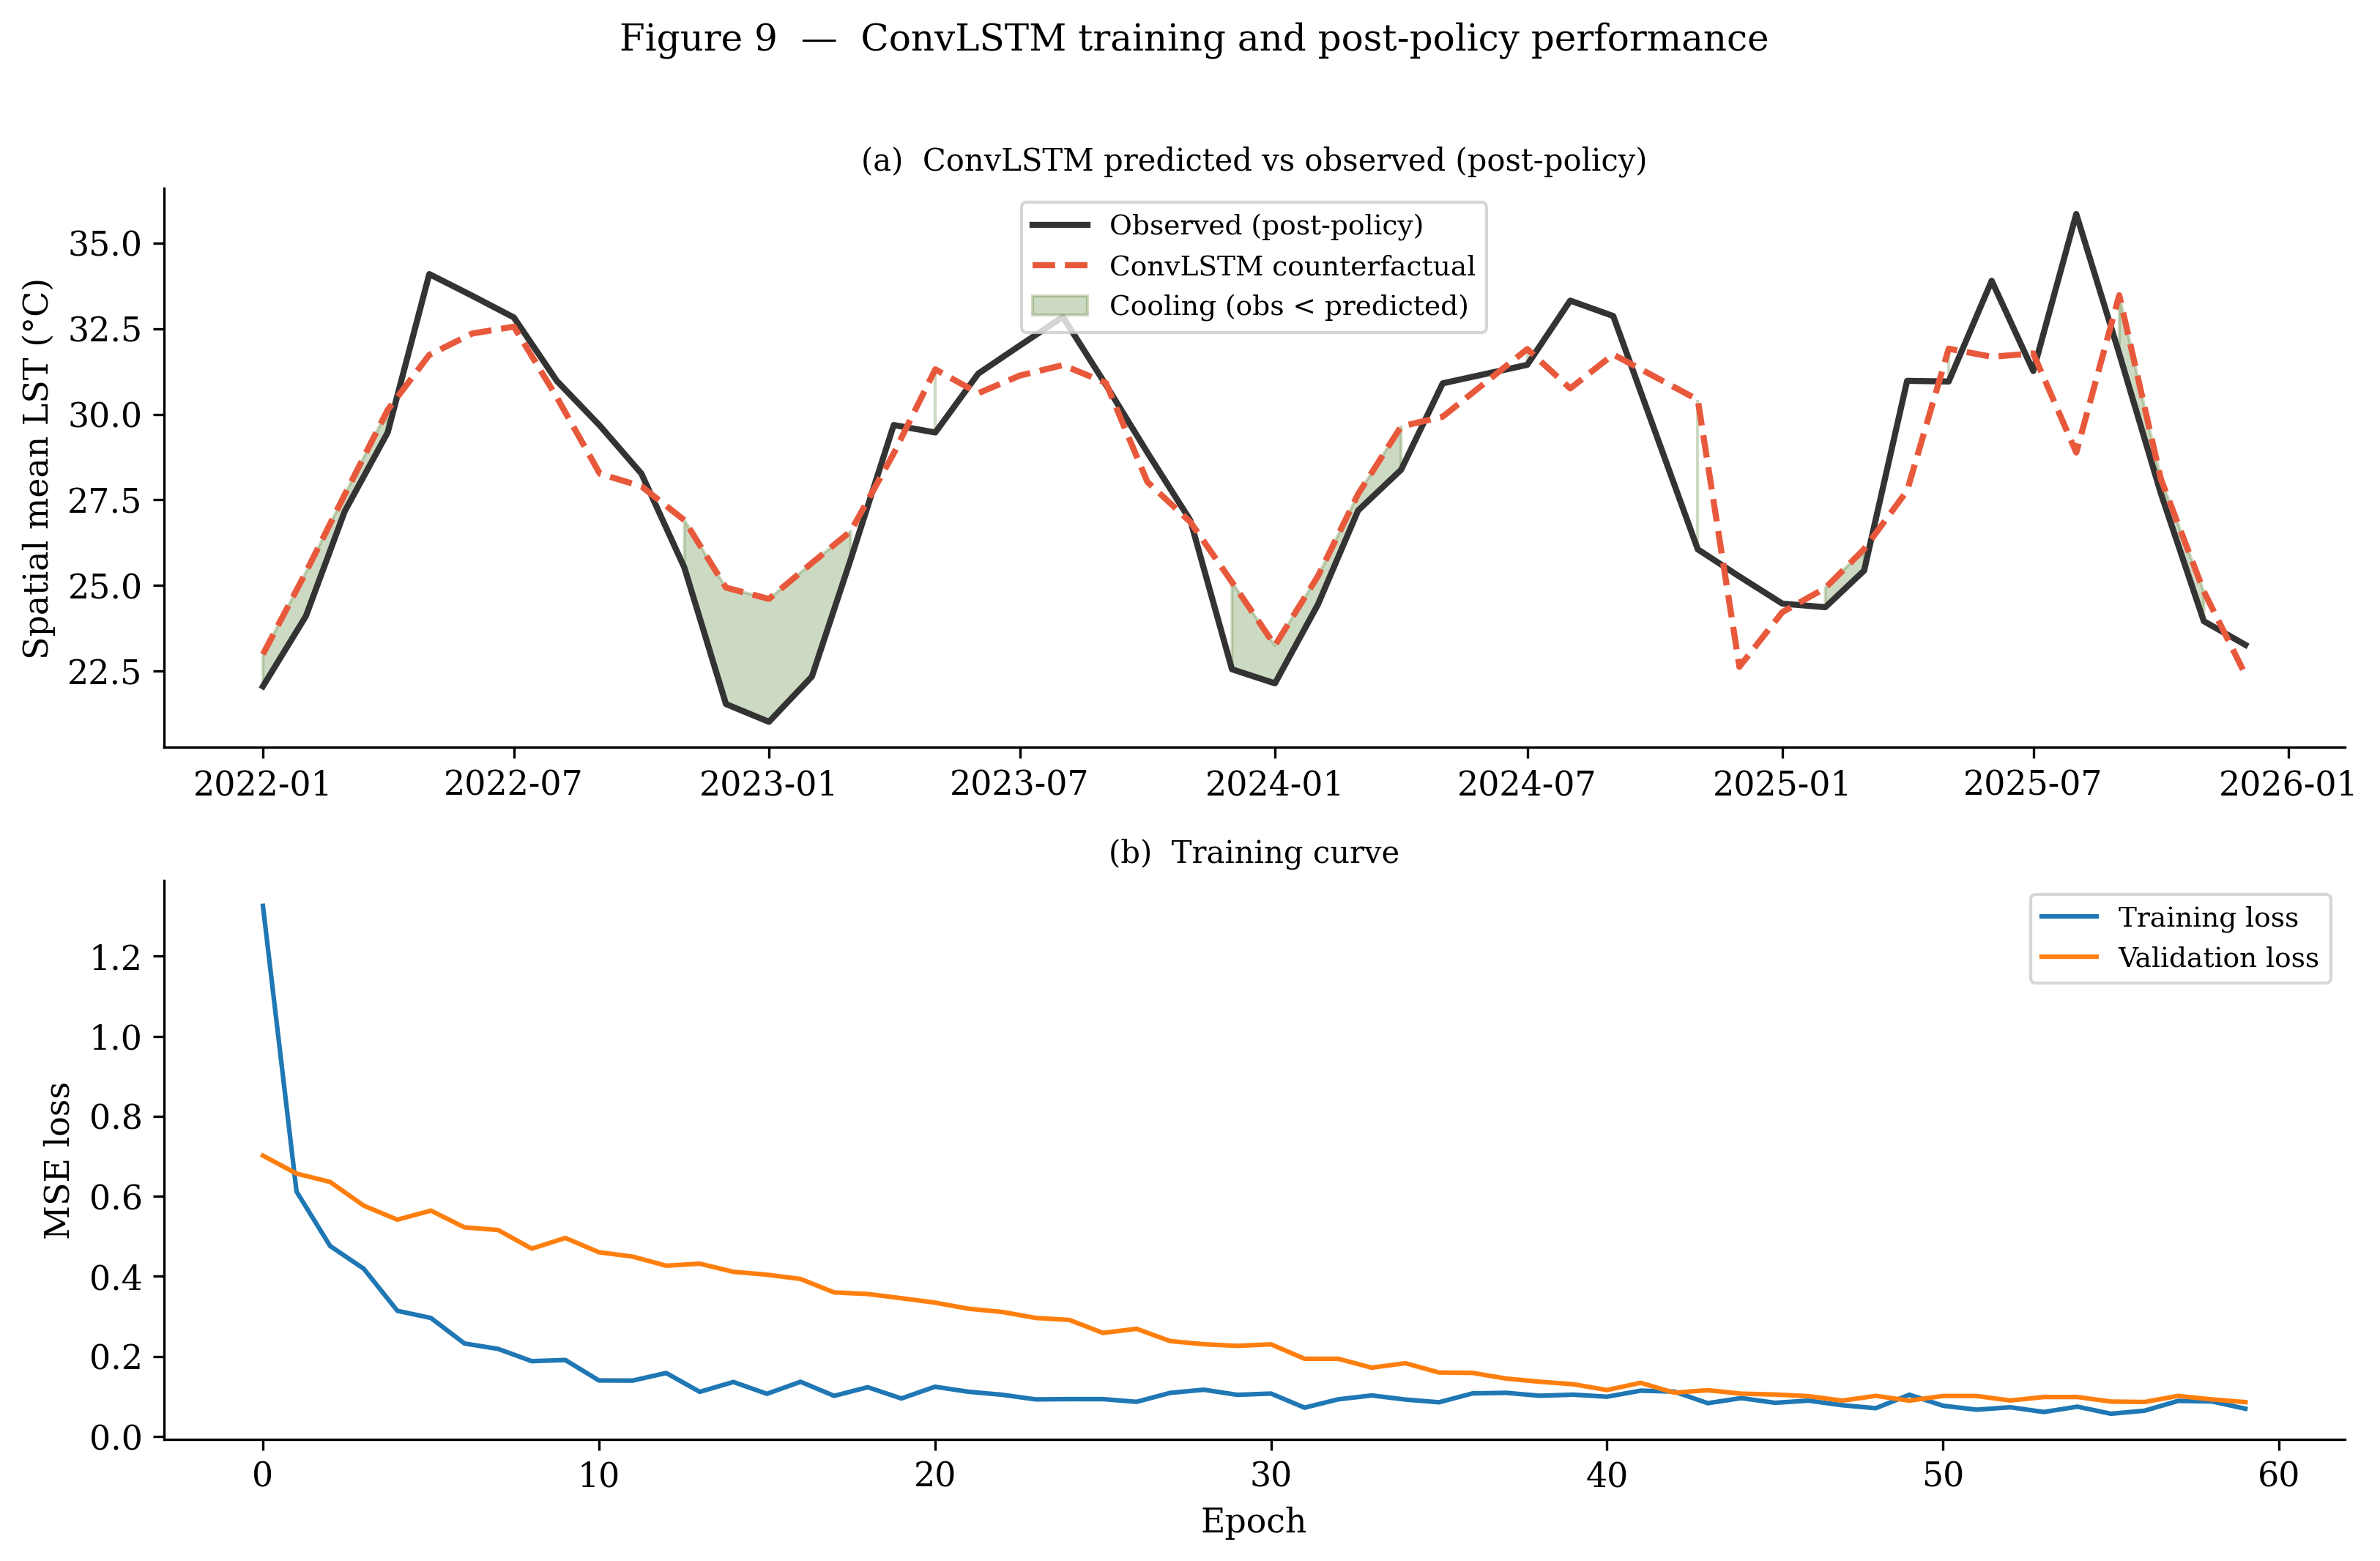
\includegraphics[width=0.68\linewidth]{fig9_convlstm_timeseries.png}
  \caption{ConvLSTM predicted vs.\ observed spatial-mean LST (top) and
  training loss curves (bottom).}
  \label{fig:convlstm_ts}
\end{figure}

\subsection{AlphaEarth Results}

The AlphaEarth analysis compares 2021 as the last full pre-policy year with
2025 as the latest available post-policy year. The mean cosine embedding change across valid cells
is 0.027, with a 90th percentile of 0.043. This indicates that most of the
city shows modest embedding movement, with a smaller number of more substantial
change hotspots.

The key question is whether locations that changed most in embedding space also
cooled. AlphaEarth cosine change is weakly positively correlated with the
ConvLSTM cooling residual ($r = 0.071$), weakly positively correlated with
annual mean $\Delta$NDVI ($r = 0.112$), and weakly negatively correlated with
annual mean $\Delta$LST ($r = -0.124$). City-wide, the annual mean LST
difference from 2021 to 2025 is +2.77$^\circ$C and the annual mean NDVI
difference is -0.0139, confirming that the broad background reflects regional
warming and slight vegetation decline.

The WorldCover-supervised classifier (Section~\ref{sec:worldcover_method})
provides a more interpretable framing. Applied to both years, it shows that the
city's AlphaEarth embeddings shifted on average toward less vegetation-like
patterns between 2021 and 2025 ($\Delta$greening\_prob $< 0$ for the majority
of cells), consistent with continued urbanization rather than widespread
greening. The correlation between $\Delta$greening\_prob and the ConvLSTM
cooling residual is near zero ($r = -0.045$), indicating that locations
where the classifier detected surface greening do not systematically overlap
with locations that cooled.

Figure~\ref{fig:quadrant_scatter} shows the point-level distribution in
$\Delta$greening\_prob versus cooling-residual space, with cells coloured by
quadrant. The greening-plus-cooling quadrant (Q1) contains only a small share
of valid cells, while cells with high greening probability change are roughly
evenly split between cooling and warming outcomes. Most cooling occurs in cells
with low or negative $\Delta$greening\_prob (Q3), suggesting that the ConvLSTM
cooling residuals in western, southwestern, and southeastern Chengdu are not primarily driven
by detectable surface greening at the current analysis resolution.

\begin{table}[t]
\caption{Key AlphaEarth alignment metrics for the 2021--2025 Chengdu comparison.}
\label{tab:alphaearth_metrics}
\centering
\small
\begin{tabular}{lc}
\toprule
\textbf{Metric} & \textbf{Value} \\
\midrule
Valid grid cells & 3298 \\
Mean cosine change & 0.0270 \\
90th percentile cosine change & 0.0425 \\
Mean Euclidean change & 0.2231 \\
$r(\text{change}, \text{cooling})$ & 0.071 \\
$r(\text{change}, \Delta LST)$ & -0.124 \\
$r(\text{change}, \Delta NDVI)$ & 0.112 \\
Mean $\Delta LST$ (2021--2025) & +2.77$^\circ$C \\
Mean $\Delta NDVI$ (2021--2025) & -0.0139 \\
\midrule
\multicolumn{2}{l}{\textit{WorldCover-supervised greening classifier}} \\
\midrule
Classifier CV accuracy & 0.758 \\
$r(\Delta\text{greening\_prob}, \text{cooling})$ & -0.045 \\
Greening + cooling overlap share (Q1) & see Fig.~\ref{fig:quadrant_scatter} \\
\bottomrule
\end{tabular}
\end{table}

\subsection{WorldCover-Supervised Greening Analysis}

The WorldCover classifier (cross-validation accuracy = 0.758) is applied to
both 2021 and 2025 AlphaEarth embeddings to produce per-cell vegetation
probability maps. The $\Delta$greening\_prob map (panel (e) of
Figure~\ref{fig:alphaearth_alignment}) is predominantly negative across the
25 km urban study area, indicating that the city's embedding patterns shifted
on average toward less vegetation-like representations between 2021 and 2025.
This is consistent with continued urban development rather than widespread
park-city greening, and aligns with the slight NDVI decline ($\Delta$NDVI
= -0.0139) observed over the same period.

The scatter of $\Delta$greening\_prob against the ConvLSTM cooling residual
(Figure~\ref{fig:quadrant_scatter}) shows a near-zero correlation
($r = -0.045$). Cells classified as greening (positive $\Delta$greening\_prob)
are roughly evenly split between the cooling and warming quadrants, while most
cells that show cooling residuals are in the paving or low-signal region.
This result clarifies the earlier finding that high-embedding-change cells are
not predominantly greening: the surface changes captured by AlphaEarth in the
post-policy period are largely consistent with urban expansion rather than
vegetation gain.

\begin{figure}[H]
  \centering
  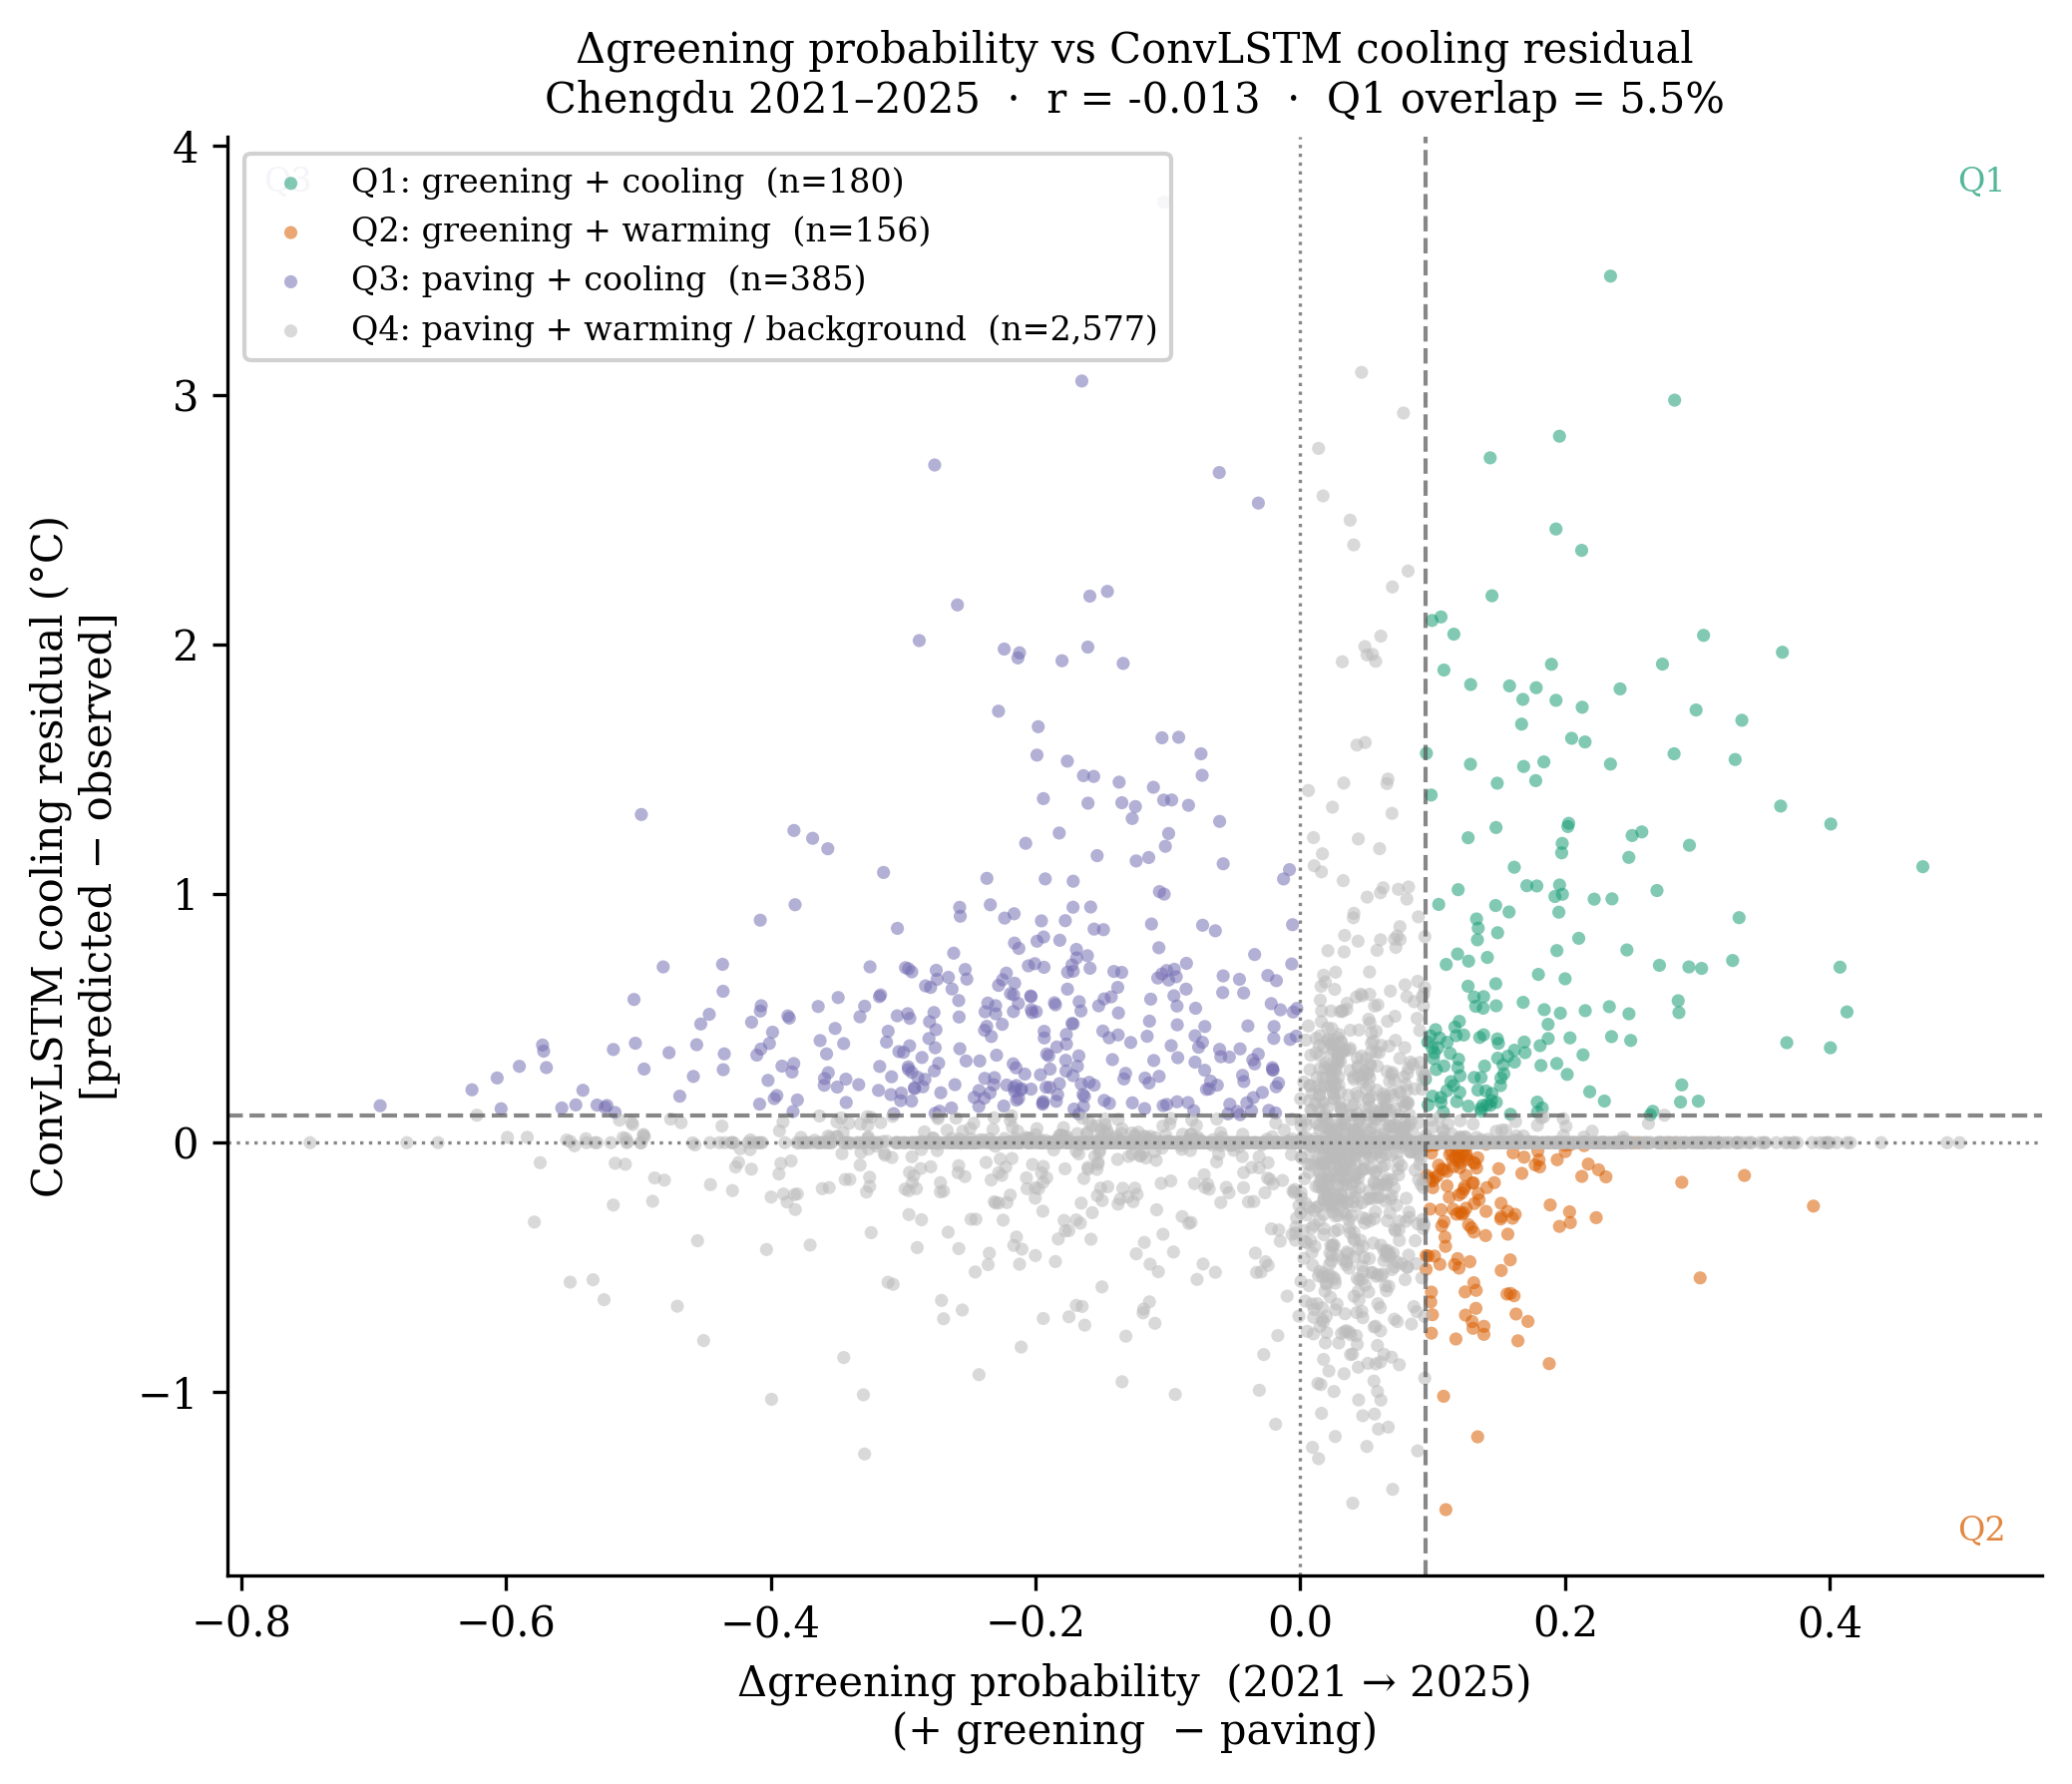
\includegraphics[width=0.72\linewidth]{chengdu_alphaearth_quadrant_scatter_2021_2025.png}
  \caption{Quadrant scatterplot of WorldCover-supervised $\Delta$greening
  probability (x-axis) versus ConvLSTM cooling residual (y-axis) for all valid
  grid cells. Points are coloured by quadrant: Q1 (green) greening and cooling;
  Q2 (orange) greening and warming; Q3 (purple) paving and cooling; Q4 (grey)
  background. Dashed lines mark the 75th-percentile thresholds for each axis;
  the dotted line marks zero on each axis.}
  \label{fig:quadrant_scatter}
\end{figure}

\begin{figure}[H]
  \centering
  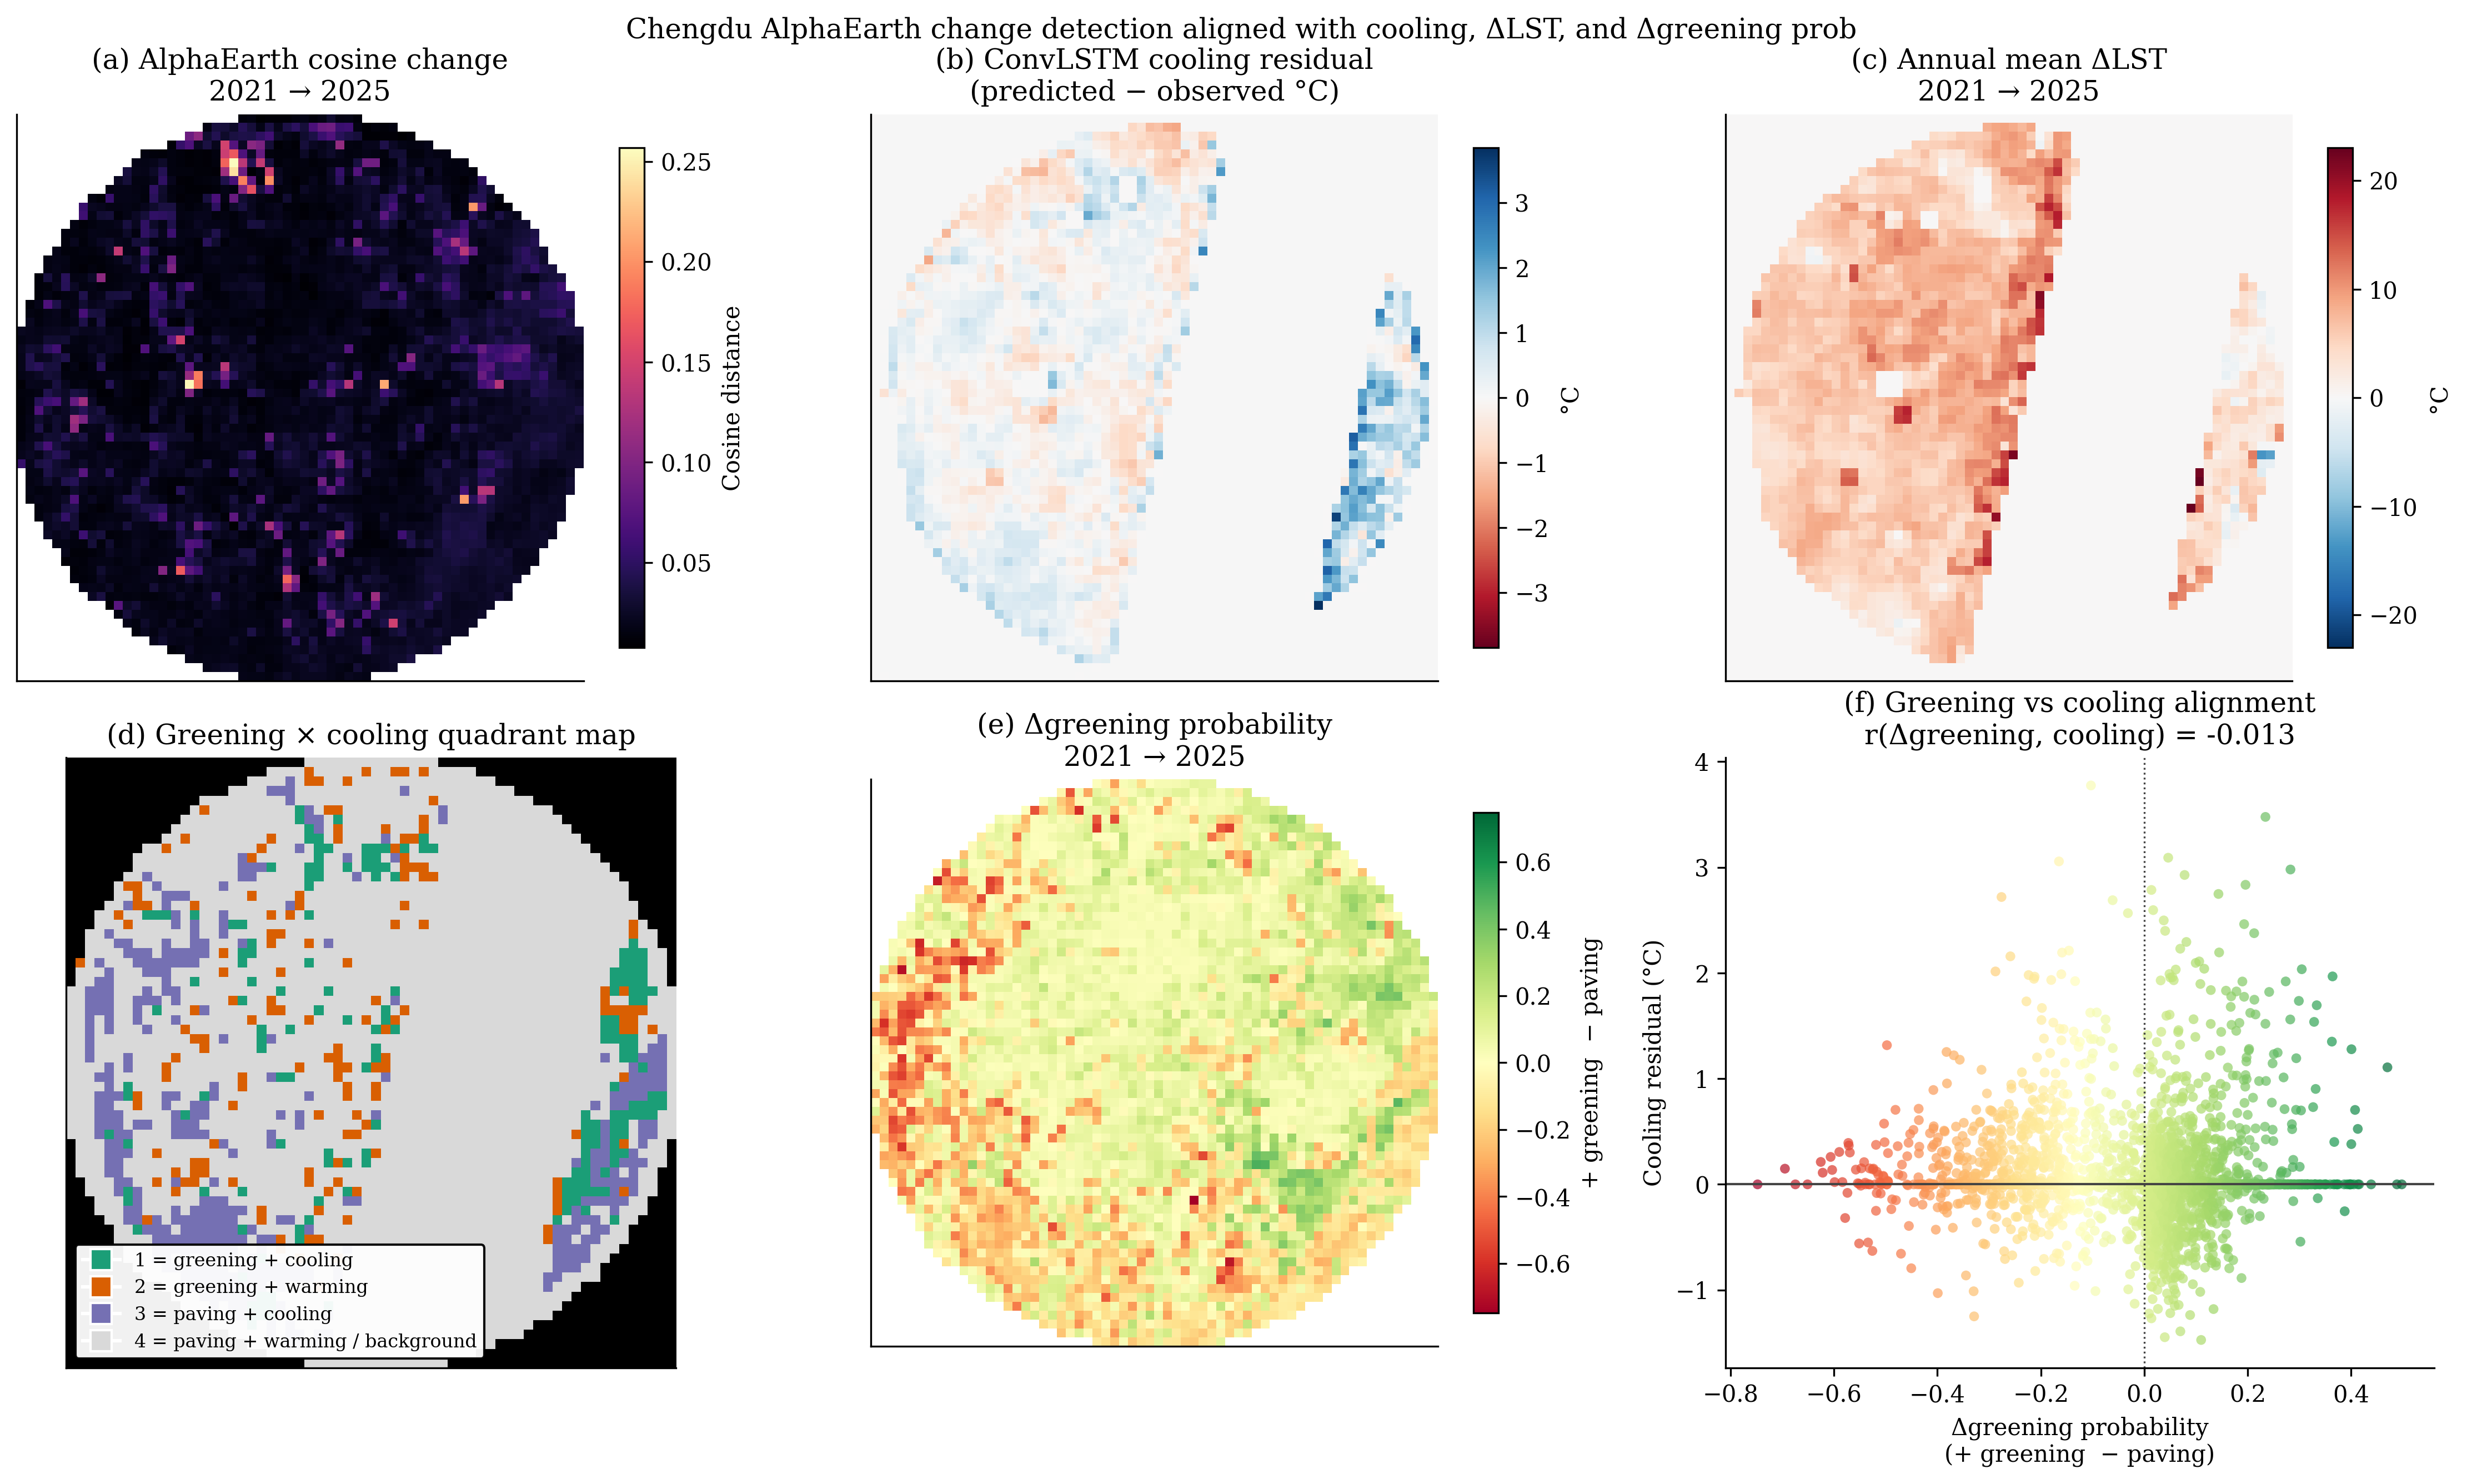
\includegraphics[width=0.80\linewidth]{chengdu_alphaearth_alignment_2021_2025.png}
  \caption{AlphaEarth alignment workflow for Chengdu. Panel (a) shows
  2021--2025 cosine embedding change. Panel (b) shows mean ConvLSTM cooling
  residual over 2022--2025. Panel (c) shows annual mean $\Delta$LST. Panel (d)
  shows the greening $\times$ cooling quadrant map: Q1 (green) greening and
  cooling; Q2 (orange) greening and warming; Q3 (purple) paving and cooling;
  Q4 (grey) background. Panel (e) shows WorldCover-supervised $\Delta$greening
  probability (positive = surface shifted toward vegetation; negative = toward
  built form). Panel (f) shows the cell-wise scatter of $\Delta$greening\_prob
  versus cooling residual. The $\Delta$LST panel contains a large
  low-information region due to incomplete Landsat coverage.}
  \label{fig:alphaearth_alignment}
\end{figure}

\FloatBarrier
\section{Discussion}
\label{sec:discussion}

\subsection{What the Chengdu Pilot Shows}

The current Chengdu results are mixed but informative. The city-wide ITS result
is weak, which suggests that the park-city policy did not create an obvious
uniform cooling signal across the whole urban area. The ConvLSTM result is more
interesting because it shows possible localized cooling zones. The AlphaEarth
extension adds a third layer: it tests whether places with thermal anomalies are
also places with measurable surface-form change.

The answer is not a simple yes. AlphaEarth embedding change shows weak
correlation with cooling ($r = 0.071$), and the WorldCover-supervised greening
classifier finds that $\Delta$greening\_prob is essentially uncorrelated with
the cooling residual ($r = -0.045$). Most cells with cooling residuals are in
the paving or low-signal quadrant, while greening cells are roughly evenly
split between cooling and warming. This makes the Chengdu pilot stronger as a
methodological demonstration than as a definitive causal case for park-city
cooling.

\subsection{Why AlphaEarth Matters}

Even with weak correlations, AlphaEarth improves the project in two ways.
First, it provides a systematic way to look for surface transformation on the
same analysis grid as the ConvLSTM residual map. Second, it forces a more
honest attribution exercise. Cooling alone is not enough. AlphaEarth makes it
possible to distinguish places that cooled and changed from places that cooled
without much detectable structural change, as well as places that changed but
warmed. In that sense, the value of the current AlphaEarth result is not that
it proves policy success, but that it provides a concrete minimum test of
whether thermal anomalies and surface change are spatially co-located.

The implemented workflow is a three-layer AI design:
\begin{enumerate}
  \item ConvLSTM detects where the thermal outcome differs from pre-policy
  expectations, identifying pixels that cooled beyond what historical
  dynamics predict.
  \item AlphaEarth cosine change detects where the physical surface changed
  in embedding space between 2021 and 2025.
  \item The WorldCover-supervised Random Forest classifier translates embedding
  change into interpretable land-cover transition probabilities, distinguishing
  greening from paving.
\end{enumerate}
The policy signal is most credible where all three layers agree: observed
cooling, positive embedding change, and a positive $\Delta$greening\_prob
pointing in the same direction. In the current Chengdu analysis, this
triple-signal overlap is limited but not absent.

\subsection{Limitations}

The main limitations are as follows. Landsat coverage is incomplete, making the
$\Delta$LST layer noisy with a large low-information zone. The post-policy
window is short, with only four years after 2021. The ConvLSTM residual and
AlphaEarth comparison are only partially aligned in time, because the embedding
change uses a 2021--2025 snapshot while the thermal residual is averaged over
2022--2025.

A critical spatial resolution constraint limits the current analysis. The
ConvLSTM model was trained at a $64 \times 64$ grid over the 25 km urban
buffer due to local computational training time constraints, yielding a cell
size of approximately 780 m. At this resolution, individual parks, greenways,
and ecological corridors (the primary intervention targets of the park-city
policy) are smaller than a single analysis cell and cannot be resolved.
Consequently, the greening-cooling alignment analysis is necessarily coarse:
a positive $\Delta$greening\_prob in a 780 m cell reflects a dominant land-cover
shift across a large area, not the addition of a specific park. Future analysis
at 30 m (Landsat) or 10 m (Sentinel-2 / AlphaEarth native) pixel resolution
would allow direct testing of whether LST decreased specifically around
documented park boundaries and greenway corridors, the ecologically
meaningful spatial unit for this policy evaluation.

\subsection{Next Step}

The most valuable next step is to move the analysis to pixel-level resolution.
Running the ConvLSTM at 30 m Landsat resolution and aligning it with the 10 m
AlphaEarth and WorldCover layers would allow direct testing of whether urban
temperatures decreased specifically in and around documented park and greenway
locations, a question the current 780 m grid cannot answer. Overlaying
official park boundary data from Chengdu's park-city planning records would
provide the ground-truth spatial units needed for this fine-scale evaluation.

\section{Conclusion}
\label{sec:conclusion}

This paper implements a three-layer AI framework for evaluating urban greening
policy in Chengdu: a ConvLSTM spatiotemporal reference to identify thermal
anomalies, AlphaEarth embedding change to detect surface transformation, and a
WorldCover-supervised Random Forest classifier to distinguish greening from
paving at the grid level.

The substantive conclusion is cautious. Chengdu still does not show a strong
city-wide cooling break after the January 2022 Park-City policy. The ConvLSTM
model suggests localized cooling residuals, and AlphaEarth shows localized
surface change hotspots, but their overlap is limited. Some of the largest
change hotspots are more consistent with warming or mixed transformation than
with cooling and vegetation gain.

That does not make AlphaEarth a failure. Instead, it makes the project more
credible. Rather than over-claiming that cooling proves policy success, the combined
workflow shows where Chengdu changed, where it cooled, and where those signals
do or do not agree, providing a more honest and actionable basis for causal
attribution than thermal analysis alone.

More broadly, the results validate the feasibility of this three-layer detection
approach. Even at the coarse 780 m grid resolution imposed by local training
constraints, the framework successfully distinguishes greening from paving,
separates thermal anomalies from background warming, and identifies where all
three signals align. This establishes a methodological foundation that can be
directly applied at higher spatial resolution. Running the same pipeline at
30 m Landsat or 10 m Sentinel-2 resolution, aligned with official park boundary
data, would allow direct testing of whether Chengdu's documented parks and
greenways produced measurable local cooling, the core policy question this
framework is designed to answer.

\FloatBarrier

\begin{thebibliography}{99}

\bibitem[Zanaga et~al.(2022)]{Zanaga2022}
Zanaga, D., Van De Kerchove, R., Daems, D., De Keersmaecker, W., Brockmann,
C., Kirches, G., Wevers, J., Cartus, O., Santoro, M., Fritz, S.,
Lesiv, M., Herold, M., Tsendbazar, N., Xu, P., Ramoino, F., \& Arino, O.
(2022).
ESA WorldCover 10 m 2021 v200.
\textit{Zenodo}.
\url{https://doi.org/10.5281/zenodo.7254221}

\bibitem[Bernal et~al.(2017)]{Bernal2017}
Bernal, J.~L., Cummins, S., \& Gasparrini, A. (2017).
Interrupted time series regression for the evaluation of public health
interventions: a tutorial.
\textit{International Journal of Epidemiology}, 46(1), 348--355.

\bibitem[Bowler et~al.(2010)]{Bowler2010}
Bowler, D.~E., Buyung-Ali, L., Knight, T.~M., \& Pullin, A.~S. (2010).
Urban greening to cool towns and cities: A systematic review of the empirical
evidence.
\textit{Landscape and Urban Planning}, 97(3), 147--155.

\bibitem[Brown et~al.(2025)]{Brown2025}
Brown, C.~F., Kazmierski, M.~R., Pasquarella, V.~J., Rucklidge, W.~J.,
Samsikova, M., Zhang, C., Shelhamer, E., Lahera, E., Wiles, O.,
Ilyushchenko, S., Gorelick, N., Zhang, L.~L., Alj, S., Schechter, E.,
Askay, S., Guinan, O., Moore, R., Boukouvalas, A., \& Kohli, P. (2025).
AlphaEarth Foundations: An embedding field model for accurate and efficient
global mapping from sparse label data.
\textit{arXiv preprint arXiv:2507.22291}.

\bibitem[Google Earth Engine(2025a)]{Google2025Catalog}
Google Earth Engine. (2025a).
Satellite Embedding V1: AlphaEarth Foundations annual embeddings.
\url{https://developers.google.com/earth-engine/datasets/catalog/GOOGLE_SATELLITE_EMBEDDING_V1_ANNUAL}

\bibitem[Google Earth Engine(2025b)]{Google2025Tutorial}
Google Earth Engine. (2025b).
Introduction to the Satellite Embedding Dataset.
\url{https://developers.google.com/earth-engine/tutorials/community/satellite-embedding-01-introduction}

\bibitem[Li et~al.(2021)]{Li2021}
Li, X., et~al. (2021).
A 40-year observation of urban expansion and urban heat island in China
assessed from satellite data.
\textit{Remote Sensing of Environment}, 215, 74--84.

\bibitem[MacKinnon \& White(1985)]{MacKinnon1985}
MacKinnon, J.~G., \& White, H. (1985).
Some heteroskedasticity-consistent covariance matrix estimators with improved
finite sample properties.
\textit{Journal of Econometrics}, 29(3), 305--325.

\bibitem[Oke(1982)]{Oke1982}
Oke, T.~R. (1982).
The energetic basis of the urban heat island.
\textit{Quarterly Journal of the Royal Meteorological Society}, 108(455),
1--24.

\bibitem[Peng et~al.(2012)]{Peng2012}
Peng, S., et~al. (2012).
Surface urban heat island across 419 global big cities.
\textit{Environmental Science \& Technology}, 46(2), 696--703.

\bibitem[Shi et~al.(2015)]{Shi2015}
Shi, X., Chen, Z., Wang, H., Yeung, D.-Y., Wong, W.-K., \& Woo, W.-C. (2015).
Convolutional LSTM network: A machine learning approach for precipitation
nowcasting.
\textit{Advances in Neural Information Processing Systems}, 28.

\bibitem[Zhao et~al.(2014)]{Zhao2014}
Zhao, L., Lee, X., Smith, R.~B., \& Oleson, K. (2014).
Strong contributions of local background climate to urban heat islands.
\textit{Nature}, 511(7508), 216--219.

\end{thebibliography}

\end{document}
